\documentclass[10pt,xcolor=dvipsnames,compress]{beamer}

\usepackage{danny_theme}
\usepackage{danny_style}
\usepackage{hyperref}
%\usepackage[algoruled,longend]{algorithm2e}
\usepackage{array}
\usepackage{graphicx}
\usepackage{amsmath}
\newcolumntype{C}{>{\centering\arraybackslash} m{1.3in} }
\newcolumntype{M}{>{\centering\arraybackslash} m{1.in} }
\everymath{\displaystyle}
\long\def\/*#1*/{}
\usepackage{multirow}

\beamertemplatenavigationsymbolsempty


%===============================================================================
% 					  Presentation Title and Author  
%===============================================================================

\title[Supercapacitor Inadequecy]{
Inadequecy Representation in\\ Models of Supercapacitor Batteries}
%\subtitle{}

\author[Danial Faghihi]{Danial Faghihi}

\institute[ICES/PECOS]{
Center for Predictive Engineering and Computational Science (PECOS)
Institute for Computational Engineering and Sciences (ICES)\\
$\quad~$The University of Texas at Austin
}

\date[Wed May 17, 2017]{PECOS Inadequecy Meeting\\
Wednesday May 17, 2017}
%===============================================================================
%===============================================================================



\begin{document}

%===============================================================================
% SLIDE 00
%===============================================================================
\begin{frame}


\includegraphics[width=.5\linewidth]{figs/grand_logo}\\
 
\titlepage
\end{frame}

%===============================================================================
% SLIDE 00
%===============================================================================
\begin{frame}
\frametitle{Outline}
\vfill

\vspace{0.7in}
\tableofcontents
\vspace{0.7in}

\vfill
\end{frame}



%%%%%%%--------------------------------------------------------------------------------------------------------------------------
\section{Summary Model Description}
%%%%%%%--------------------------------------------------------------------------------------------------------------------------
%===============================================================================
% SLIDE 00
%===============================================================================
\begin{frame}
\frametitle{Outline}
\vfill

\vspace{0.7in}
\tableofcontents[currentsection,currentsubsection] 
\vspace{0.7in}

\vfill
\end{frame}


%===============================================================================
% SLIDE 03
%===============================================================================
\begin{frame}
\frametitle{Governing Equations}
\vfill

\begin{columns}
\begin{column}{.65\textwidth}
\begin{block}{electrode}
\textbf{Current density} following Ohm's law:
\begin{itemize}
\item Matrix phase :
$
\mathbf{i}_1 = -\sigma\nabla\phi_1
$
\item Solution phase:
$
\mathbf{i}_2 = -\kappa\nabla\phi_2
$
\end{itemize}
$\phi_1$, $\phi_2$: potentials,\\
$\sigma$, $\kappa$: electronic/ionic conductivity.
%

\vspace{0.1in}
\textbf{Conservation of charge:}
\vspace{-0.1in}
\begin{equation*}
-\nabla \cdot \mathbf{i}_1 =  \nabla\cdot \mathbf{i}_2 = a {i}_n
\vspace{-0.1in}
\end{equation*}
$a$: interfacial area per unit volume \\
${i}_n$: current transferred from the matrix to the electrolyte\\
$
{i}_n = \underbrace{C \frac{\partial}{\partial t} \blue{\eta}}_{\rm double-layer} +
\underbrace{{i}_0 ( \exp (\frac{\alpha_aF}{RT} \blue{\eta}) - \exp (-\frac{\alpha_cF}{RT}\blue{\eta})}_{\rm faradaic})
$

\vspace{0.07in}
\begin{center}
overpotential: 
$
\blue{\eta =  \phi_1 - \phi_2}
$
\end{center}

\end{block}
\end{column}
%-----------------------------
\begin{column}{.30\textwidth} 
\begin{center}
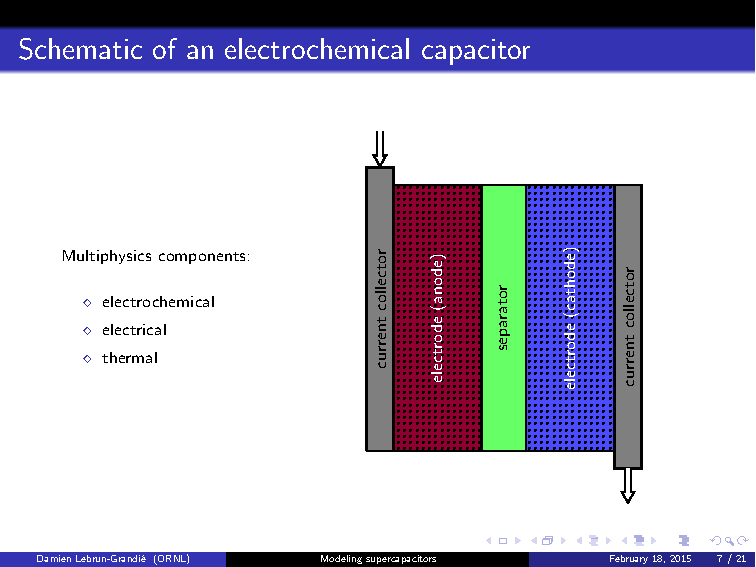
\includegraphics[trim = 2.4in 0.42in 0.7in 0.9in, clip, width=.7\textwidth]{figs/supercap_schematic.pdf}  
\end{center}
\begin{block}{collector}
\begin{equation*}
\mathbf{i}_1 = -\sigma\nabla\phi_1
\end{equation*}
\begin{equation*}
-\nabla \cdot \mathbf{i}_1 = 0
\end{equation*}
\end{block}
%%
\begin{block}{seperator}
\begin{equation*}
\mathbf{i}_2 = -\kappa\nabla\phi_2
\end{equation*}
\begin{equation*}
-\nabla \cdot \mathbf{i}_2 = 0
\end{equation*}
\end{block}
\end{column}
\end{columns}


\vfill
\end{frame}


%===============================================================================
% Slide 04
%===============================================================================
\begin{frame}
\frametitle{High Fidelity Model}
\vfill

\begin{columns}
\begin{column}{.47\textwidth} 
	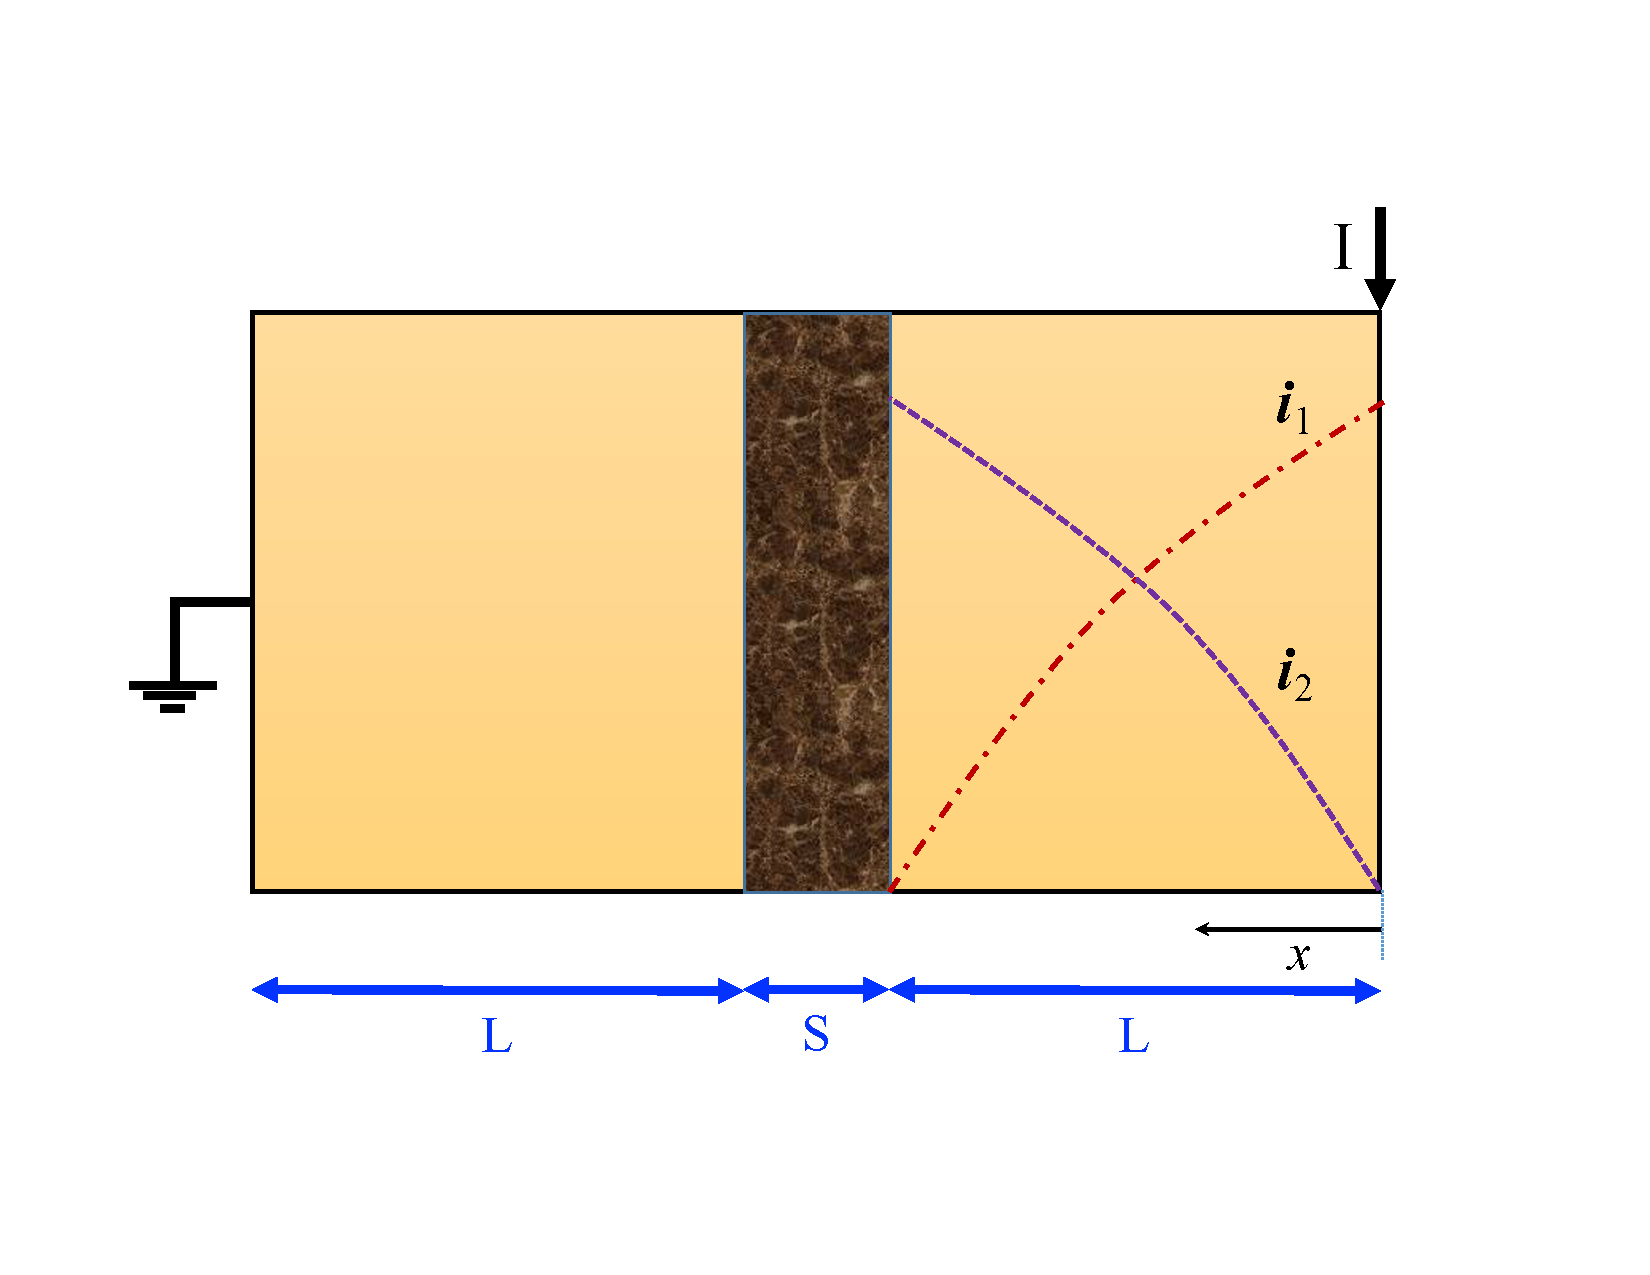
\includegraphics[trim = 0in 1.4in 0in 1.4in, clip, width=1\textwidth]{figs/schematic.pdf}
\end{column}
%-----------------------------
\begin{column}{.47\textwidth}
\begin{itemize}
\begin{small}
\item $\eta(\xi,\tau)$ = overpotential in electrode\\
\item $\gamma = \frac{\kappa}{\sigma}$ : conductivity ratio \\
\item $\xi, \tau$ : dimensionless distance/time \\
\item $I(\tau)$ : dimensionless current
\end{small}
\end{itemize}
\end{column}
\end{columns}
%%====================
\begin{columns}
\begin{column}{.47\textwidth}
\vspace{-0.1in}
\begin{alertblock}{Modeling Assumptions (Sins)}
\begin{enumerate}[i.]

\begin{footnotesize}
\item No Faradaic processes:
current transferred from matrix to the solution phase goes towards only charging the double-layer at the electrode/electrolyte interface.

\item $\phi_1$ is uniformly distributed over the current collector domain (collector is sufficiently thin)
%
%The electrical resistivity of the current collector is low (or it is sufficiently thin) that one can assume uniform distribution of $\phi_1$ over the collector domain: \textit{homogeneous in the $x$-direction}, 

\item There is no electron/ion fluxes cross the top and bottom boundaries
%. Also due to high conductivity of collectors, the voltage over the whole interface on the collector side is negligible (similar to case that tab on the left collector is grounded): \textit{2D domain could be reduced to a quasi-1D domain},

\item The material properties are constant within each layer
\end{footnotesize}

\end{enumerate}
\end{alertblock}
\end{column}
%-----------------------------
\begin{column}{.47\textwidth}
\begin{problock}{High Fidelity model}
\begin{equation*}\label{eq:HF}
\frac{\partial\eta}{\partial\tau} = \frac{\partial^2\eta}{\partial\xi^2}
\end{equation*}
\begin{equation*}
\left\{\begin{matrix}
\frac{\partial\eta}{\partial\xi}|_{\xi=0} & = & -\frac{\gamma}{1+\gamma}I(\tau)\\
\frac{\partial\eta}{\partial\xi}|_{\xi=1} & = & \frac{1}{1+\gamma}I(\tau) \nonumber\\
\eta|_{\tau=0} 					       & =  & \eta_0(\xi)
\end{matrix}\right.
\end{equation*}
\end{problock}
\end{column}
%-----------------------------

\end{columns}


\vfill
\end{frame}


%===============================================================================
% Slide 05
%===============================================================================
\begin{frame}
\frametitle{Low Fidelity Model}
\vfill


\begin{alertblock}{Modeling Assumptions (Sin)}
\begin{enumerate}[i.]

\item Assuming a quadratically varying profile for overpotential inside the electrodes
\begin{equation*}\label{eq:quadratic}
\eta_{LF} (\xi,\tau)= a(\tau)\xi^2 + b(\tau)\xi + c(\tau)
\end{equation*}
where $a$, $b$, and $c$ can be obtained from PDE+BCs of HF model.

\end{enumerate}
\end{alertblock}

%-----------------------------
\begin{block}{Low Fidelity model}
\begin{equation*}\label{eq:LF}
\eta_{LF}(\xi,\tau) = 
\frac{1}{2}I(\tau)\xi^2 - I(\tau) \frac{\gamma}{1+\gamma}\xi + {\eta}^{avg}(\tau) - \frac{I(\tau)}{6} + \frac{I(\tau)}{2}\frac{\gamma}{1+\gamma}
\end{equation*}
${\eta}^{avg}$ is the solution of following ODE given appropriate initial condition:
\begin{equation*}\label{eq:LF_avg}
\frac{\partial{\eta}^{avg}}{\partial\tau} = I(\tau)
\end{equation*}
%
where $\eta^{avg}$ is the spatial
average of the governing equation over the entire domain length
%
$
\eta^{avg} = \int_0^1 \eta d\xi 
$
\end{block}


\vfill
\end{frame}



%===============================================================================
% Slide 06
%===============================================================================
\begin{frame}
\frametitle{QoI : cell voltage }
\vfill


\begin{alertblock}{Quantity of Interest}
 Potential drop across the system
 \begin{eqnarray*}
 V^{\rm cell}(\tau) &=& \phi_{\rm collector}^L - \phi_{\rm collector}^R \\
 		&=& 2V_0 - 2V^{\rm elect.} - V^{\rm sep.}
 \end{eqnarray*}

where 

$
V^{\rm elect.}(\tau) =  \phi_{\rm 1}|_{\xi=0} - \phi_{\rm 2}|_{\xi=1} = \frac{1+2\gamma}{1+\gamma}\eta|_{\xi=1} - \frac{\gamma}{1+\gamma}\eta|_{\xi=0} 
 - \frac{\gamma}{(1+\gamma)^2}I
$

and

$
V^{\rm sep.}(\tau) =  
I\frac{L_s}{\kappa_s}
$

\end{alertblock}



\vfill
\end{frame}



%%%%%%%--------------------------------------------------------------------------------------------------------------------------
\section{Inadequecy Representation}
%%%%%%%--------------------------------------------------------------------------------------------------------------------------
%===============================================================================
% SLIDE 00
%===============================================================================
\begin{frame}
\frametitle{Outline}
\vfill

\vspace{0.7in}
\tableofcontents[currentsection,currentsubsection] 
\vspace{0.7in}

\vfill
\end{frame}


%===============================================================================
% Slide 07
%===============================================================================
\begin{frame}
\frametitle{Inadequacy Representation: Objective}
\vfill


\begin{alertblock}{Objective:}
Based on what we know about the models, develop a representation of inadequacy (\textit{error in QoI}, $\epsilon$) as a parametric model $\mathcal{P}(\boldsymbol{\theta})$ such that 
\begin{equation*}
V^{\rm cell}_{\rm HF} \equiv  V^{\rm cell}_{\rm LF} + \epsilon
\end{equation*}
\end{alertblock}


\begin{itemize}

\item Parameters of inadequacy model, $\boldsymbol{\theta}$, needs to be calibrated using the data furnished by HF model for simple scenarios, e.g. 

\begin{figure}[h]
    \centering
    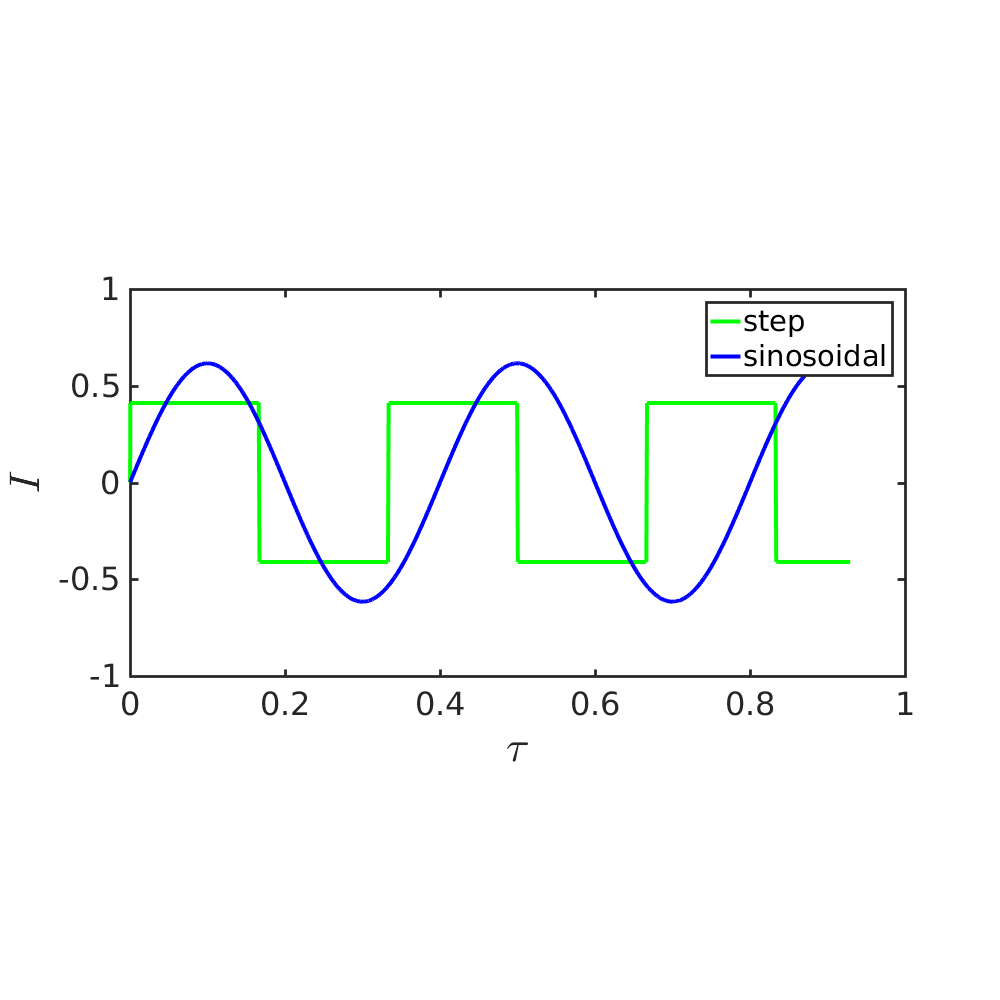
\includegraphics[trim = 0.in 2.4in 0.8in 2.8in, clip, width=0.5\textwidth]{figs/I_scenario.png} 
\end{figure}

\vspace{-0.1in}

\item $\mathcal{P}(\boldsymbol{\theta})$ enables predicting $V^{\rm cell}$ for more complex scenarios outside the HF data domain along with the associated uncertainty.

\end{itemize}


\vfill
\end{frame}



%===============================================================================
% Slide 07
%===============================================================================
\begin{frame}
\frametitle{Inadequacy Representation}
\vfill


Inadequacy model $\mathcal{P}(\boldsymbol{\theta})$ involves:
\begin{itemize}
\item \textit{Deterministic counterpart:}
Encapsulates our information about the models.

\item \textit{Stochastic counterpart:}
Represents the remaining uncertainty due to lack of information about features of full HF system.
\end{itemize}

\begin{columns}
\column{0.25\textwidth}
\begin{figure}[h]
    \centering
    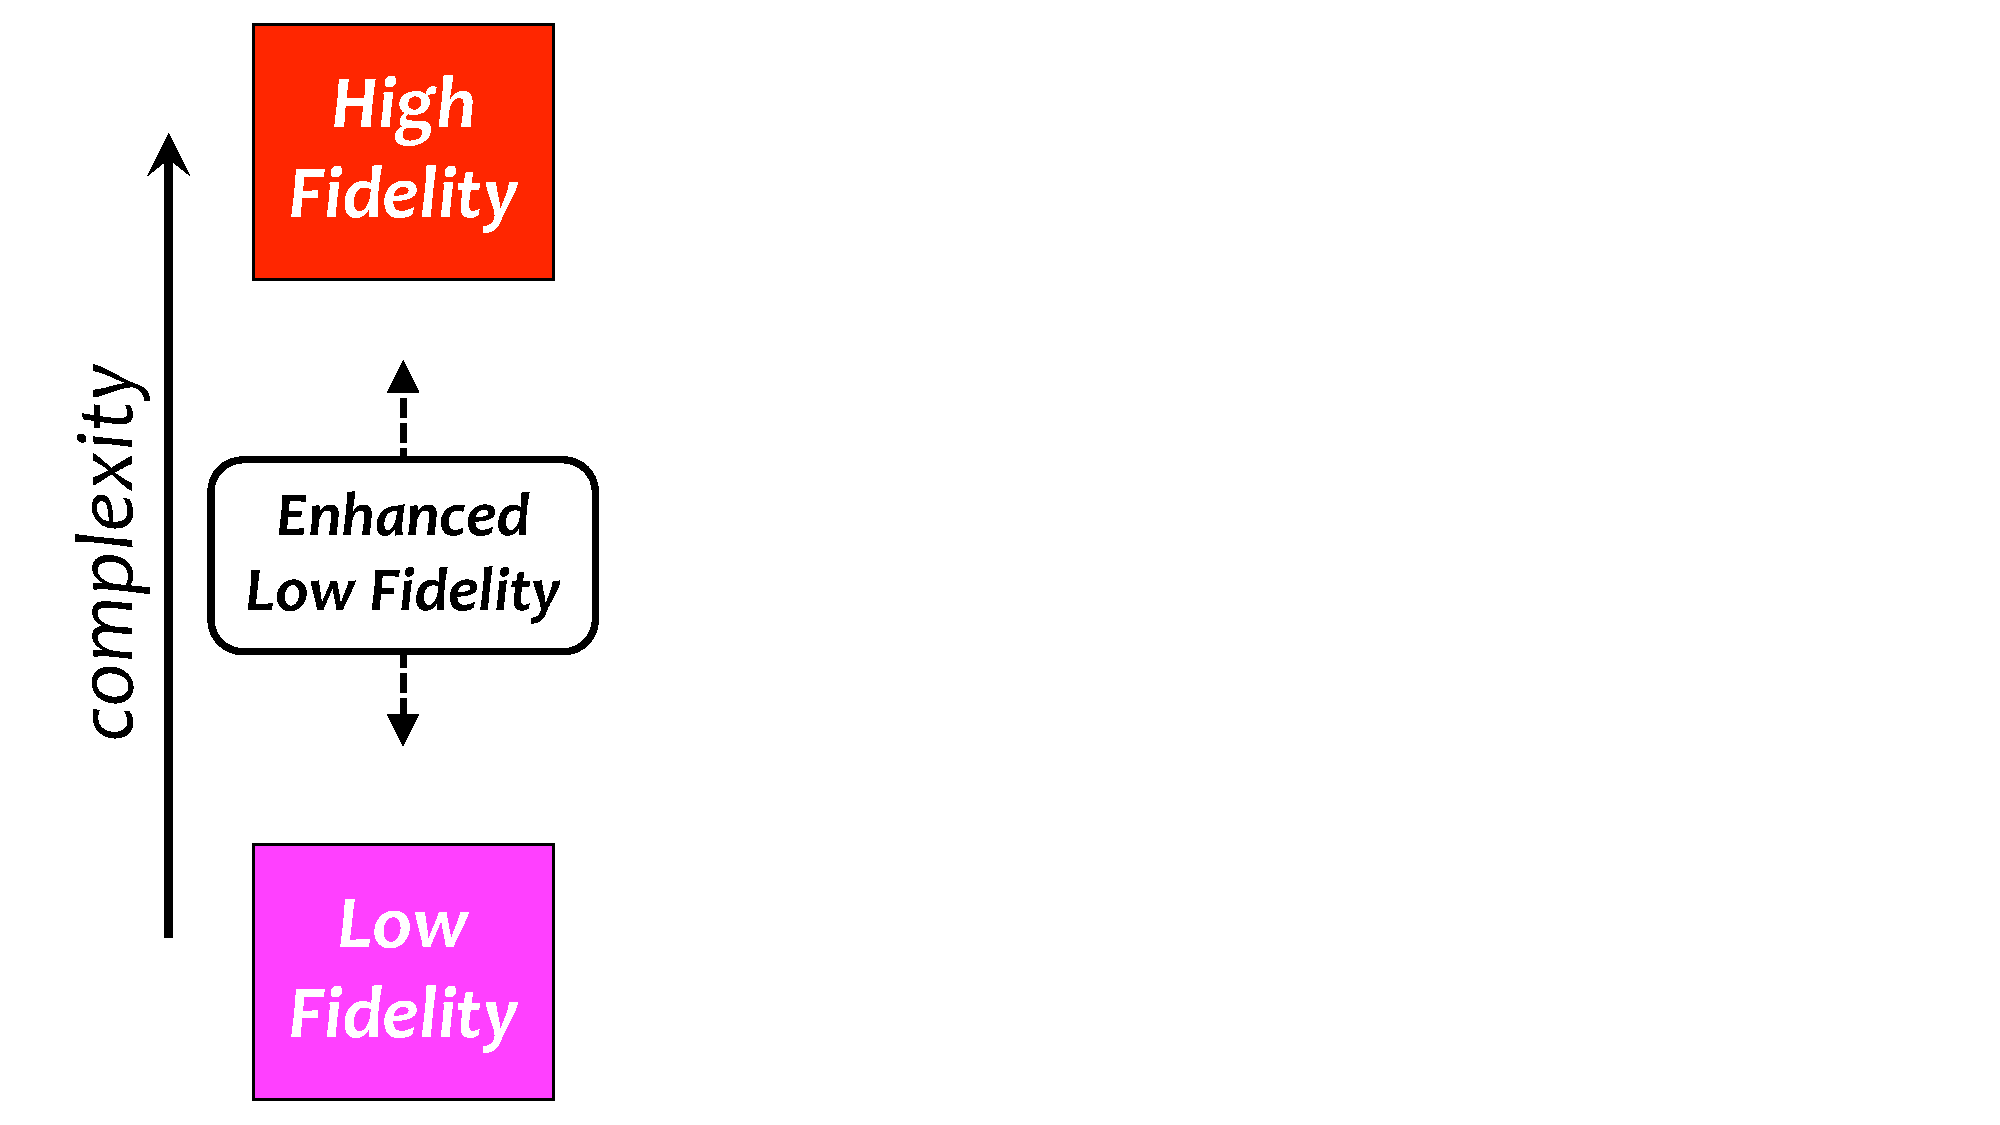
\includegraphics[trim = 0.in 0.in 9.in 0in, clip, width=1\textwidth]{figs/ELFmodel.pdf} 
\end{figure}

\column{0.75\textwidth}

\begin{block}{}

\begin{itemize}
\item The goal is to identify a set $\mathcal{M}$ of enhanced low fidelity (ELF) models, with increasing complexity,  based on our knowledge about the system, 
\vspace{-0.1in}
\begin{equation*}
\mathcal{M} = \{\mathcal{P}_1(\boldsymbol{\theta}_1), \mathcal{P}_2(\boldsymbol{\theta}_2), \cdots, \mathcal{P}_n(\boldsymbol{\theta}_n)  \},
\vspace{-0.1in}
\end{equation*}

each model class have its own parameter space ($\boldsymbol{\theta}_k \in \Theta_k$). Thus,

\begin{itemize}
\item Deterministic $\mathcal{P}^{\rm d}(\boldsymbol{\theta}^{\rm d})$ :
$\epsilon^{\rm d} = V^{\rm cell}_{\rm ELF} -  V^{\rm cell}_{\rm LF}$
\item Stochastic $\mathcal{P}^{\rm s}(\boldsymbol{\theta}^{\rm s})$: 
$\epsilon^{\rm s} = V^{\rm cell}_{\rm HLF} -  V^{\rm cell}_{\rm ELF}$
\end{itemize}


\item The more complex ELF model:
\begin{itemize}
\item more complex deterministic $\mathcal{P}^{\rm d}$ i.e. more parameters
\item more HF data might be required to calibrate 
\item less uncertainty in prediction.
\end{itemize}

\end{itemize}
\end{block}


\end{columns}


\vfill
\end{frame}


%===============================================================================
% Slide 01
%===============================================================================
\begin{frame}
\frametitle{Summary of Models and QoI}
\vfill

\begin{columns}
\begin{column}{.35\textwidth} 
\begin{problock}{HF model}

\begin{equation*}\label{eq:HF}
\frac{\partial\eta}{\partial\tau} = \frac{\partial^2\eta}{\partial\xi^2}
\end{equation*}
\begin{equation*}
\left\{\begin{matrix}
\frac{\partial\eta}{\partial\xi}|_{\xi=0} = & -\frac{\gamma I}{1+\gamma}\\
\frac{\partial\eta}{\partial\xi}|_{\xi=1} = & \frac{I}{1+\gamma} \nonumber\\
\eta|_{\tau=0} 	 =  & \eta_0(\xi)
\end{matrix}\right.
\end{equation*}

\end{problock}
\end{column}
%-----------------------------
\begin{column}{.6\textwidth}
\begin{block}{LF model}
\begin{eqnarray*}
\eta = 
\frac{1}{2}I\xi^2 - \frac{I \gamma}{1+\gamma}\xi +
{\eta}^{avg}(\tau) - \frac{I}{6} + \frac{I\gamma}{2(1+\gamma)}
\end{eqnarray*}
%
\textbf{QoI:}
$
V_{\rm LF}(\tau) = {\eta}^{avg}(\tau) + C_{\rm LF} I(\tau)
$
where
\begin{equation*}
\frac{\partial{\eta}^{avg}}{\partial\tau} = I(\tau)
\end{equation*}
\end{block}

\end{column}
\end{columns}


\begin{center}
\textbf{What do we know about HF and LF models?}
\end{center}

\begin{itemize}
\item Governing equations of HF and LF and the assumptions made to build LF model.
\item Model responses in simple cases, e.g. simplified BCs, constant current. 
\item Any other mathematical/physical information that does not require full solution of HF.


\end{itemize}



\vfill
\end{frame}



%===============================================================================
% Slide 01
%===============================================================================
\begin{frame}
\frametitle{Knowledge about the models}
\vfill


\begin{problock}{}
\begin{enumerate}

\item HF model is a PDE with \textit{infinite dimensional} solution space (i.e. function space) while  
LF model is an ODEs having a \textit{finite dimensional} state vector. 

%The solution to an ordinary differential equation, of order n, can be written as a linear combination of n independent solutions, with n undetermined constants- a vector space of dimension n. 
%The solution to a partial differential equation, of order n, can be written as a linear combination of n independent solutions but with n undetermined functions. The functions themselves constitute an infinite dimensional vector space.

\item \textbf{Constant current case:} asymptotic behavior of HF is equivalent to LF, i.e. solution of LF converges to HF after a certain time.
\begin{center}
    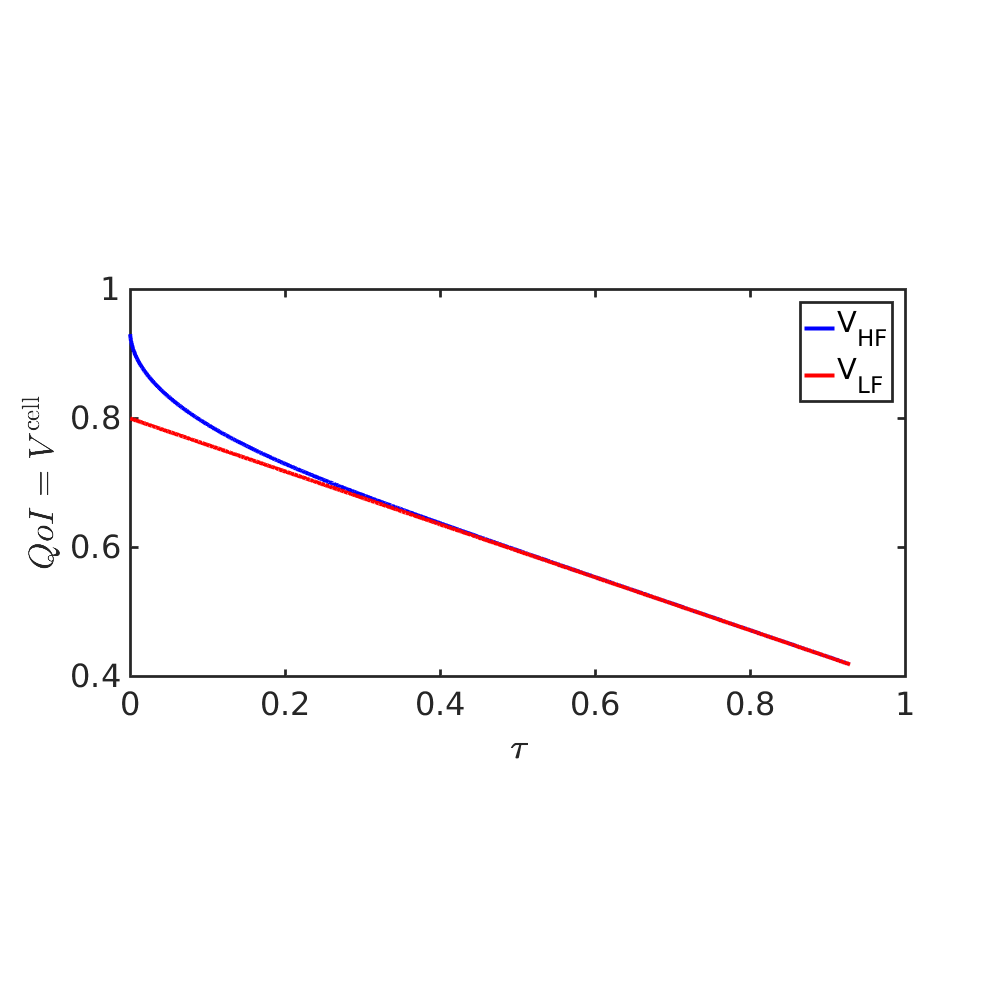
\includegraphics[trim = 0.in 2.4in 0.in 2.8in, clip, width=0.3\textwidth]{figs/Iconst_V_hf_lf.png} 

\end{center}

\item HF model response dependent on the entire current history, $I(\tau)$, up to time $\tau$. Such history does not appear with right dependency in LF model.

\textit{One way to prove this property is through thermodynamics consistency of HF model and Principles of Fading Memory}\footnote{
Coleman, B.D. and E. H. Dill., 1971. Thermodynamic restrictions on the constitutive equations of electromagnetic theory.}$^,$\footnote{
Coleman, B.D. and Noll, W., 1961. Foundations of linear viscoelasticity.}. 
 

\end{enumerate}
\end{problock}


\vfill
\end{frame}


%%%%%%%--------------------------------------------------------------------------------------------------------------------------
\subsection{Constructing ELF model}
%===============================================================================
% SLIDE 00
%===============================================================================
\begin{frame}
\frametitle{Outline}
\vfill

\vspace{0.7in}
\tableofcontents[currentsection,currentsubsection] 
\vspace{0.7in}

\vfill
\end{frame}


%===============================================================================
% Slide 01
%===============================================================================
\begin{frame}
\frametitle{Constructing ELF model: higher order polynomial}
\vfill

One way to construct ELF is using higher order polynomial functions to approximate the spatial distribution of overpotential. 

Subramanian et al.\footnote{Subramanian, V. R., Ritter, J. A., and White, R. E. (2001). Approximate solutions for galvanostatic discharge of spherical particles i. constant diffusion coefficient. Journal of The Electrochemical Society, 148(11), E444-E449.}
compared the exact solution of a similar PDE+BCs with 2nd, 4th, and 6th order polynomial approximations.
\begin{figure}
    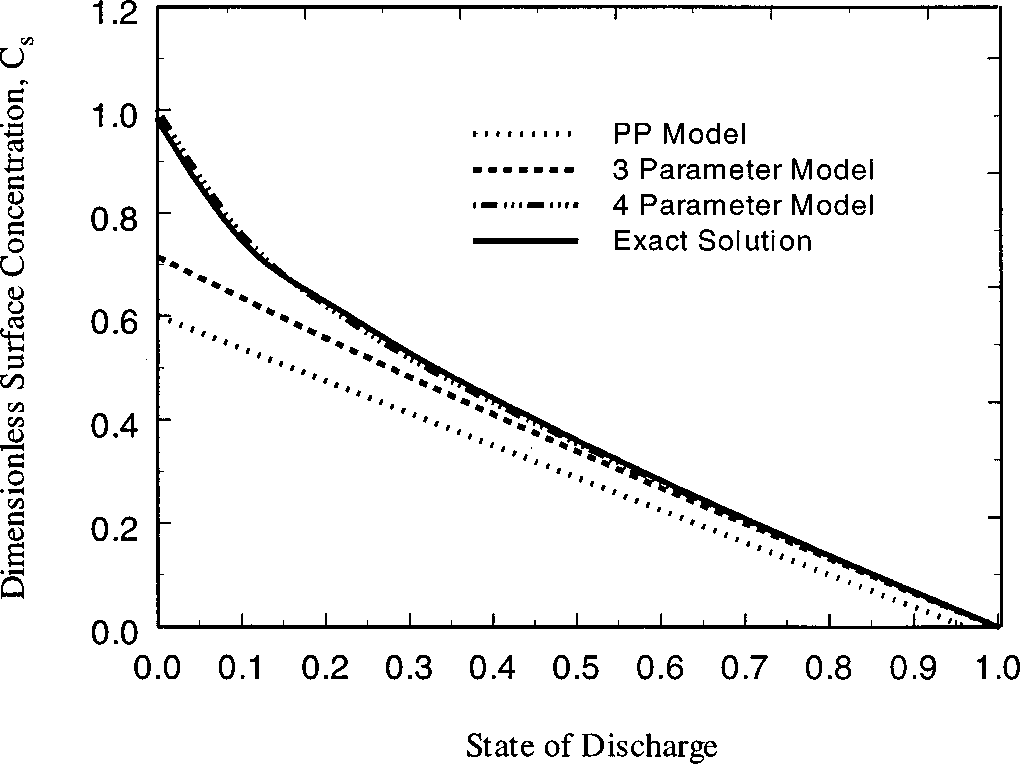
\includegraphics[trim = 0.in 0.in 0.in 0.in, clip, width=0.5\textwidth]{figs/sub.png} 
\end{figure}



\vfill
\end{frame}


%===============================================================================
% Slide 01
%===============================================================================
\begin{frame}
\frametitle{Constructing ELF model: DDE}
\vfill


\textbf{Delay Differential Equations (DDEs):}


\begin{itemize}
\item DDEs are a large and important class of dynamical systems. They
often employed in control problems in which a delay (naturally or technologically) arises between the observation and
the control action.


\item A simple form of DDEs is an ODE with deviation,
$
\mathbf{x}'(t) = \mathbf{f}(t,\mathbf{x}(t), \mathbf{x}(t-\tau)), \; \tau>0
$
, where $\tau$ is a constant time delay.


\item ODEs require specifying \textit{initial conditions}, i.e. a small set of numbers indicating the initial values of the state variables at $t_0$.

To solve a DDE at every time step, we need to specify an \textit{initial function} $\phi(t), t_0-\tau \leq t \leq t_0$ which gives the behavior of the system prior to $t_0$.


\item DDEs are \textit{infinite dimensional}:

To initialize a DDE one must specify the value of state variable over an entire interval (an infinite number of points), thus the manifold of solutions for arbitrary $\phi(t)$ is infinite-dimensional.

% another way to look at this is through Taylor expansion around t=tau that requires infinite number of initial conditions.

\end{itemize}



\vfill
\end{frame}



%===============================================================================
% Slide 01
%===============================================================================
\begin{frame}
\frametitle{Constructing ELF model}
\vfill


\begin{block}{LF model}
$
V_{\rm LF}(\tau) = {\eta}^{avg}(\tau) + C_{\rm LF} I(\tau)
$
; \quad
$
\frac{\partial{\eta}^{avg}}{\partial\tau} = I(\tau), \; {\eta}^{avg}(0)=0, \;  \tau>0 
$
\end{block}

In real system (HF model) the cell potential supposedly reacts not in an instantaneous way to the change in current.

We enhance the LF model by creating a delay equation (DDE) and introducing a constant time delay $t_s
$:



\begin{alertblock}{ELF model}
$
V_{\rm ELF}(\tau) = \hat{\eta}(\tau) + C_{\rm ELF} I(\tau - t_s)
$
; \quad
$
\frac{\partial{\hat{\eta}}}{\partial\tau} = I(\tau- t_s), \; {\hat{\eta}}(0)=0, \;  \tau>0
$
\begin{center}
$
{\rm Initial \; Finction:\;} I(\tau)=\phi(\tau), \;  -t_s \leq \tau \leq 0
$
\end{center}
\end{alertblock}


\begin{enumerate}
\item The ELF model (DDEs) belong to the class of systems with the functional state, similar to PDEs are infinite dimensional. 

\item ELF model, to some extend, bring the history information of the current.

\item The asymptotic behavior of ELF model is equivalent to LF and HF models.

\end{enumerate}


\vfill
\end{frame}


%%%%%%%--------------------------------------------------------------------------------------------------------------------------
\subsection{Deterministic part of inadequacy}
%===============================================================================
% SLIDE 00
%===============================================================================
\begin{frame}
\frametitle{Outline}
\vfill

\vspace{0.7in}
\tableofcontents[currentsection,currentsubsection] 
\vspace{0.7in}

\vfill
\end{frame}

%===============================================================================
% Slide 01
%===============================================================================
\begin{frame}
\frametitle{Inadequacy Representation: Deterministic}
\vfill

\begin{itemize}
\item Deterministic  $\mathcal{P}^{\rm d}(\boldsymbol{\theta})$ :
$\epsilon^{\rm d}  = 	V^{\rm cell}_{\rm ELF} -  V^{\rm cell}_{\rm LF}$

\item The objective is not to solve the full ELF system, rather using it to motivates a mathematical form for inadequacy model.

\item Using Taylor expansion:
\begin{equation*}
V_{\rm ELF}(\tau) = \hat{\eta}(\tau) + C_{\rm ELF} \left(
I(\tau) - t_s \frac{\partial I}{\partial \tau} + \frac{1}{2} t_s^2 \frac{\partial^2 I}{\partial \tau^2} + \cdots
\right)
\end{equation*}
 with
\begin{equation*}
\frac{\partial{\hat{\eta}}}{\partial\tau} = I(\tau) - t  \frac{\partial^2{\hat{\eta}}}{\partial\tau^2} - \frac{1}{2} t_s^2 \frac{\partial^3{\hat{\eta}}}{\partial\tau^3} + \cdots
\end{equation*}


\item One can increase the complexity of the ELF and corresponding $\mathcal{P}^{\rm d}$ by considering more Taylor expansion terms.

\end{itemize}



\vfill
\end{frame}


%===============================================================================
% Slide 01
%===============================================================================
\begin{frame}
\frametitle{Inadequacy Representation: Deterministic}
\vfill


Constructing $\mathcal{P}_1^{\rm d}(\boldsymbol{\theta})$ using one Taylor expansion term of ELF: 

\begin{equation*}
V_{\rm LF} = {\eta}^{avg} + C_{\rm LF} I
\quad {\rm with} \quad 
\frac{\partial{{\eta}^{avg}}}{\partial\tau} = I
\end{equation*}

\begin{equation*}
V_{\rm ELF} = \hat{\eta} + C_{\rm ELF} (
I - t_s \frac{\partial I}{\partial \tau}
)
\quad {\rm with} \quad 
\frac{\partial{\hat{\eta}}}{\partial\tau} = I - t_s  \frac{\partial^2{\hat{\eta}}}{\partial\tau^2}
\end{equation*}

Substituting above relations in $\epsilon_1^{\rm d} = V_{\rm ELF}- V_{\rm LF}$ and evaluating $\frac{\partial\epsilon_1^{\rm d}}{\partial\tau}$ and little manipulation, one can derive:

\begin{block}{}

\begin{equation*}
\mathcal{P}_1^{\rm d}(\boldsymbol{\theta}_1^{\rm d}) : \quad
\frac{\partial\epsilon_1^{\rm d}}{\partial\tau} + \lambda^2\epsilon_1^{\rm d} = \alpha \frac{\partial I}{\partial\tau} + \beta I
\end{equation*}
\\where $
\boldsymbol{\theta}_1^{\rm d}=
(\lambda, \alpha, \beta)
$ needs to be calibrated against HF data.

\end{block}

\vfill
\end{frame}


%===============================================================================
% Slide 01
%===============================================================================
\begin{frame}
\frametitle{Inadequacy Representation: Deterministic}
\vfill


Using second terms of the Taylor expansions, and following similar derivation, motivates an inadequacy representation such as:

\begin{problock}{}

\begin{equation*}
\mathcal{P}_2^{\rm d}(\boldsymbol{\theta}_2^{\rm d}) : \quad
\frac{\partial^2\epsilon_2^{\rm d}}{\partial\tau^2} + \lambda^2\frac{\partial\epsilon_2^{\rm d}}{\partial\tau} + \mu^2\epsilon_2
^{\rm d} =  \alpha I + \beta \frac{\partial I}{\partial\tau} + 
\rho \frac{\partial^2 I}{\partial\tau^2}
\end{equation*}

\end{problock}

writing the above relation as system of 1st order ODEs

\begin{problock}{}

\begin{equation*}
\mathcal{P}_2^{\rm d}(\boldsymbol{\theta}_2^{\rm d}) :\left\{\begin{matrix}
 x_1'(\tau) = & x_2(\tau) &\\ 
x_2'(\tau) = & \mathcal{I}(\tau) &-\mu^2 x_1(\tau) - \lambda^2 x_2(\tau)
\end{matrix}\right.
\end{equation*}
where $\epsilon_2^{\rm d} = x_1(\tau)$ \\
and
$\mathcal{I}(\tau) = \alpha I + \beta \frac{\partial I}{\partial \tau} + \rho \frac{\partial^2 I}{\partial \tau^2}$\\

where $
\boldsymbol{\theta}_2^{\rm d}=
(\lambda, \mu, \alpha, \beta, \rho)
$ needs to be calibrated against HF data.

\end{problock}


\vfill
\end{frame}



%===============================================================================
% Slide 01
%===============================================================================
\begin{frame}
\frametitle{Inadequacy Representation: Deterministic}
\vfill


\textbf{Constant current case:}

Under constant current assumption, it can be easily shown that

\begin{equation*}
V_{\rm ELF}  \equiv V_{\rm LF} + \sum_{i = 1}^n C_i \exp(-\frac{\tau}{t_i})
\end{equation*}

where number of terms in the Prony series $n$ determine the complexity of the ELF model.

Also, it is trivial
 to prove that $V_{\rm ELF} \rightarrow V_{\rm HF}$ as $n \rightarrow \infty$.

\vspace{0.1in}
Calibrating against HF data:
\vspace{-0.1in}
\begin{figure}
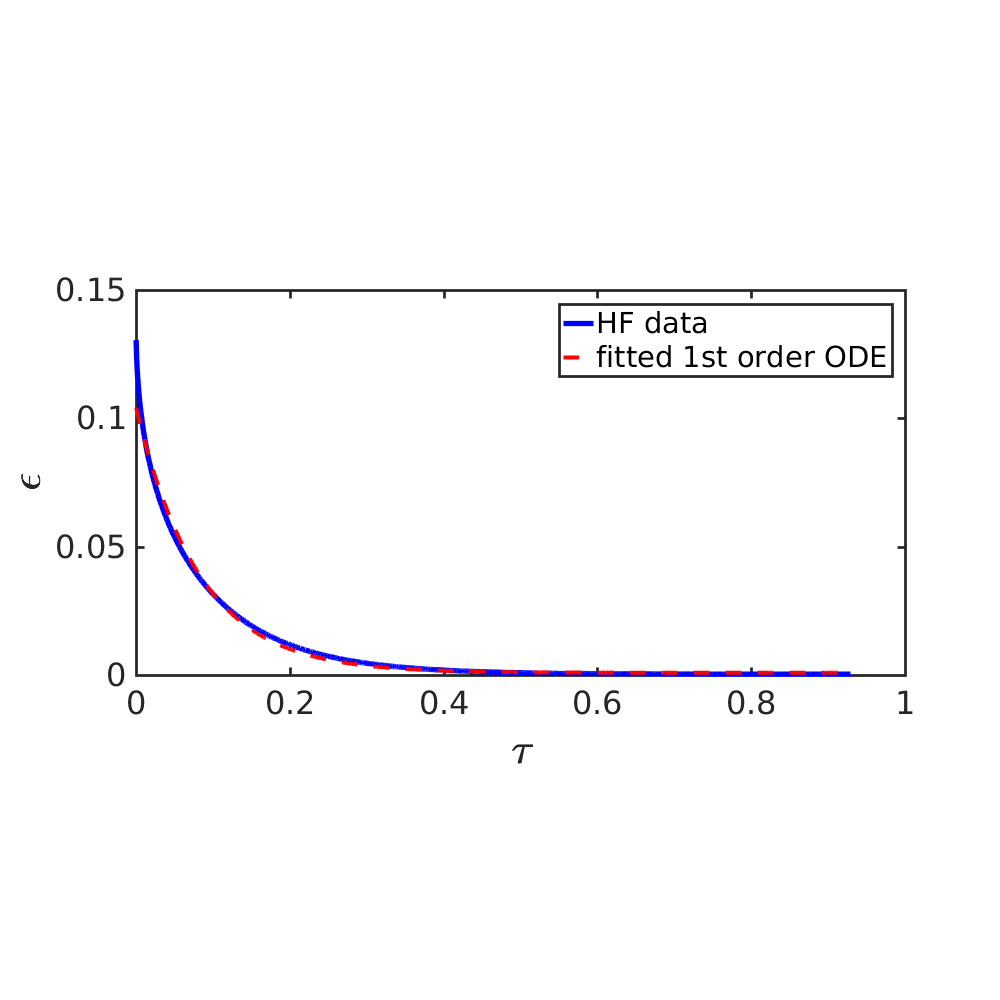
\includegraphics[trim = 0.in 2.4in 0.in 2.8in, clip, width=0.5\textwidth]{figs/Iconst_eps_modelfit_1st.png}
~
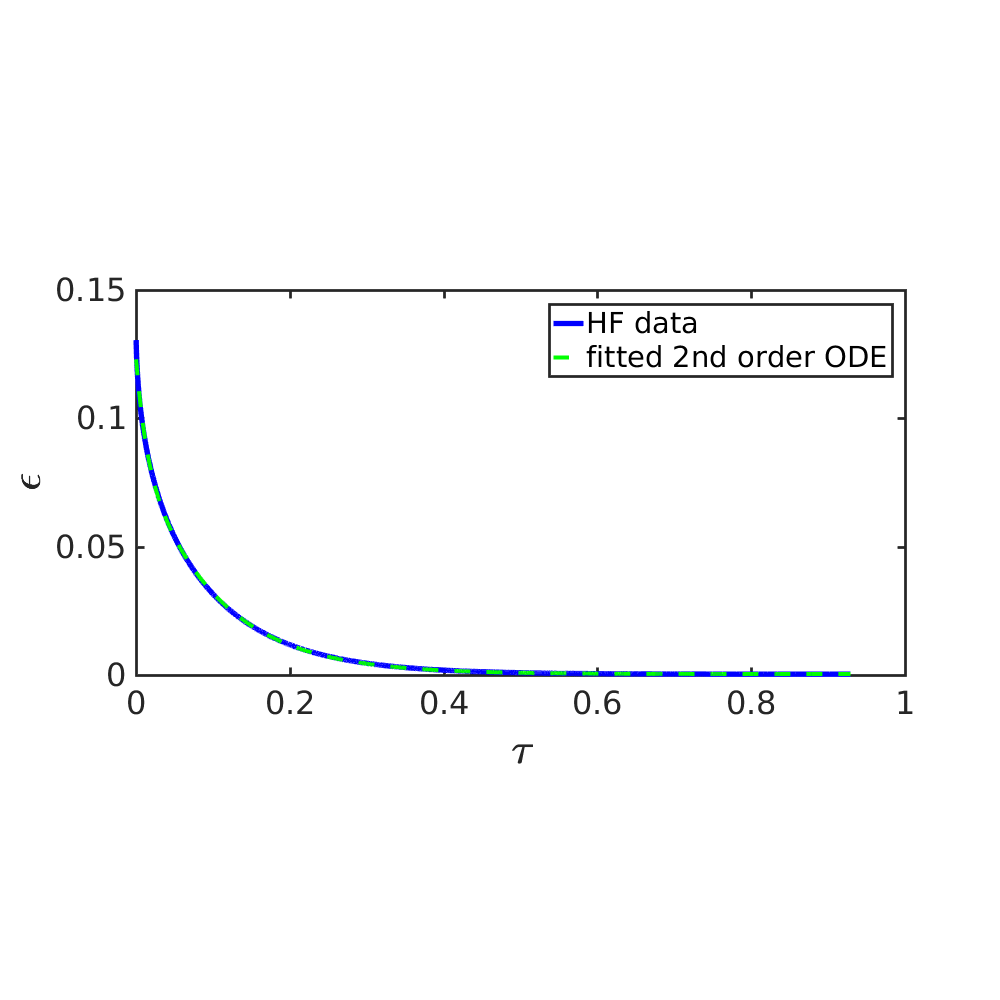
\includegraphics[trim = 0.in 2.4in 0.in 2.8in, clip, width=0.5\textwidth]{figs/Iconst_eps_modelfit_2nd.png}
\end{figure}


\vfill
\end{frame}


%===============================================================================
% Slide 01
%===============================================================================
\begin{frame}
\frametitle{Inadequacy Representation: Deterministic}
\vfill


\textbf{Constant current case:}


Calibrating inadequacy models against HF data: \\
$\mathcal{P}_1^{\rm d}:   \lambda = 3.47, \beta = 0.0223 \qquad$
$\mathcal{P}_2^{\rm d}:   \lambda = 9.55, \mu = 28.82, \alpha = 0.532$


If finite number of exponential decay enhancements, $n$, is taken into account for constructing ELF, the motivated inadequacy model is incapable of capturing HF data in a small time scale.
\vspace{-0.2in}
\begin{figure}
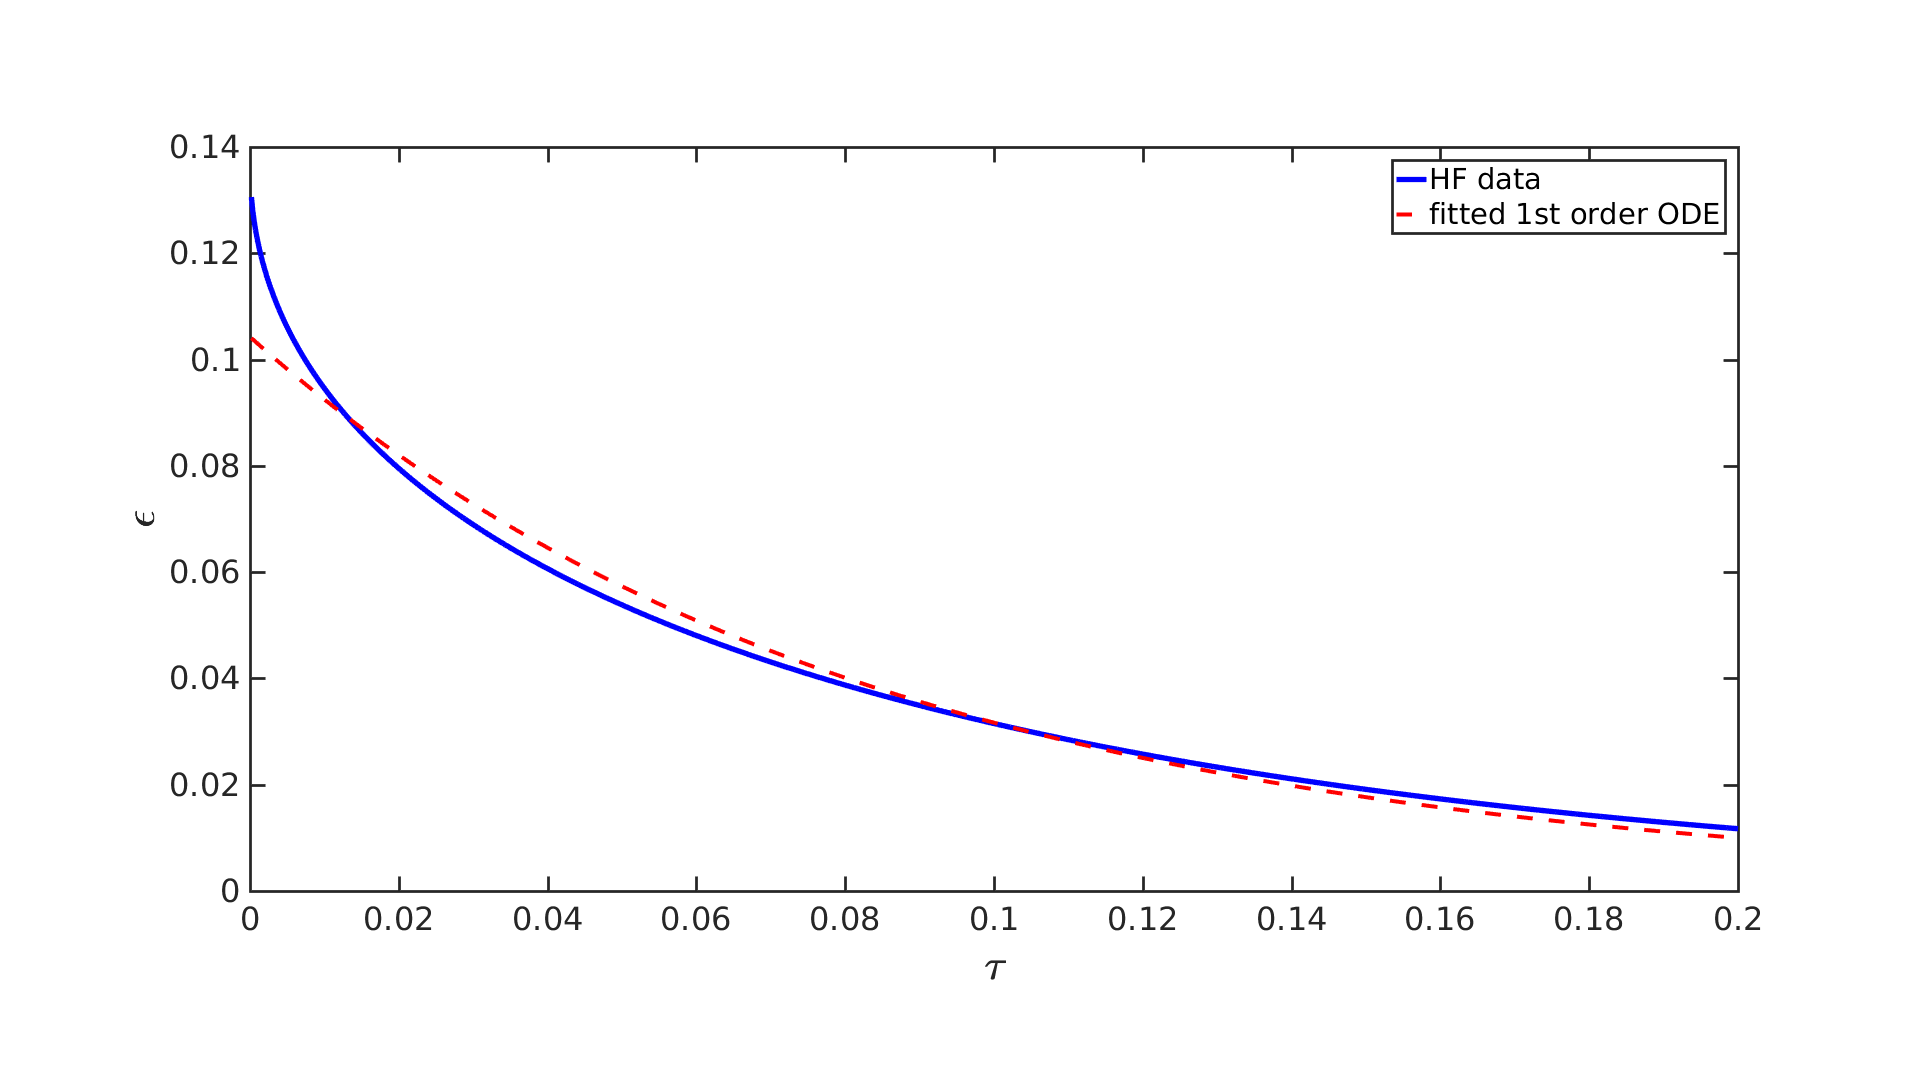
\includegraphics[trim = 1.in 1.in 1.in 1.3in, clip, width=0.5\textwidth]{figs/Iconst_eps_modelfit_1st_zoom.png}
~
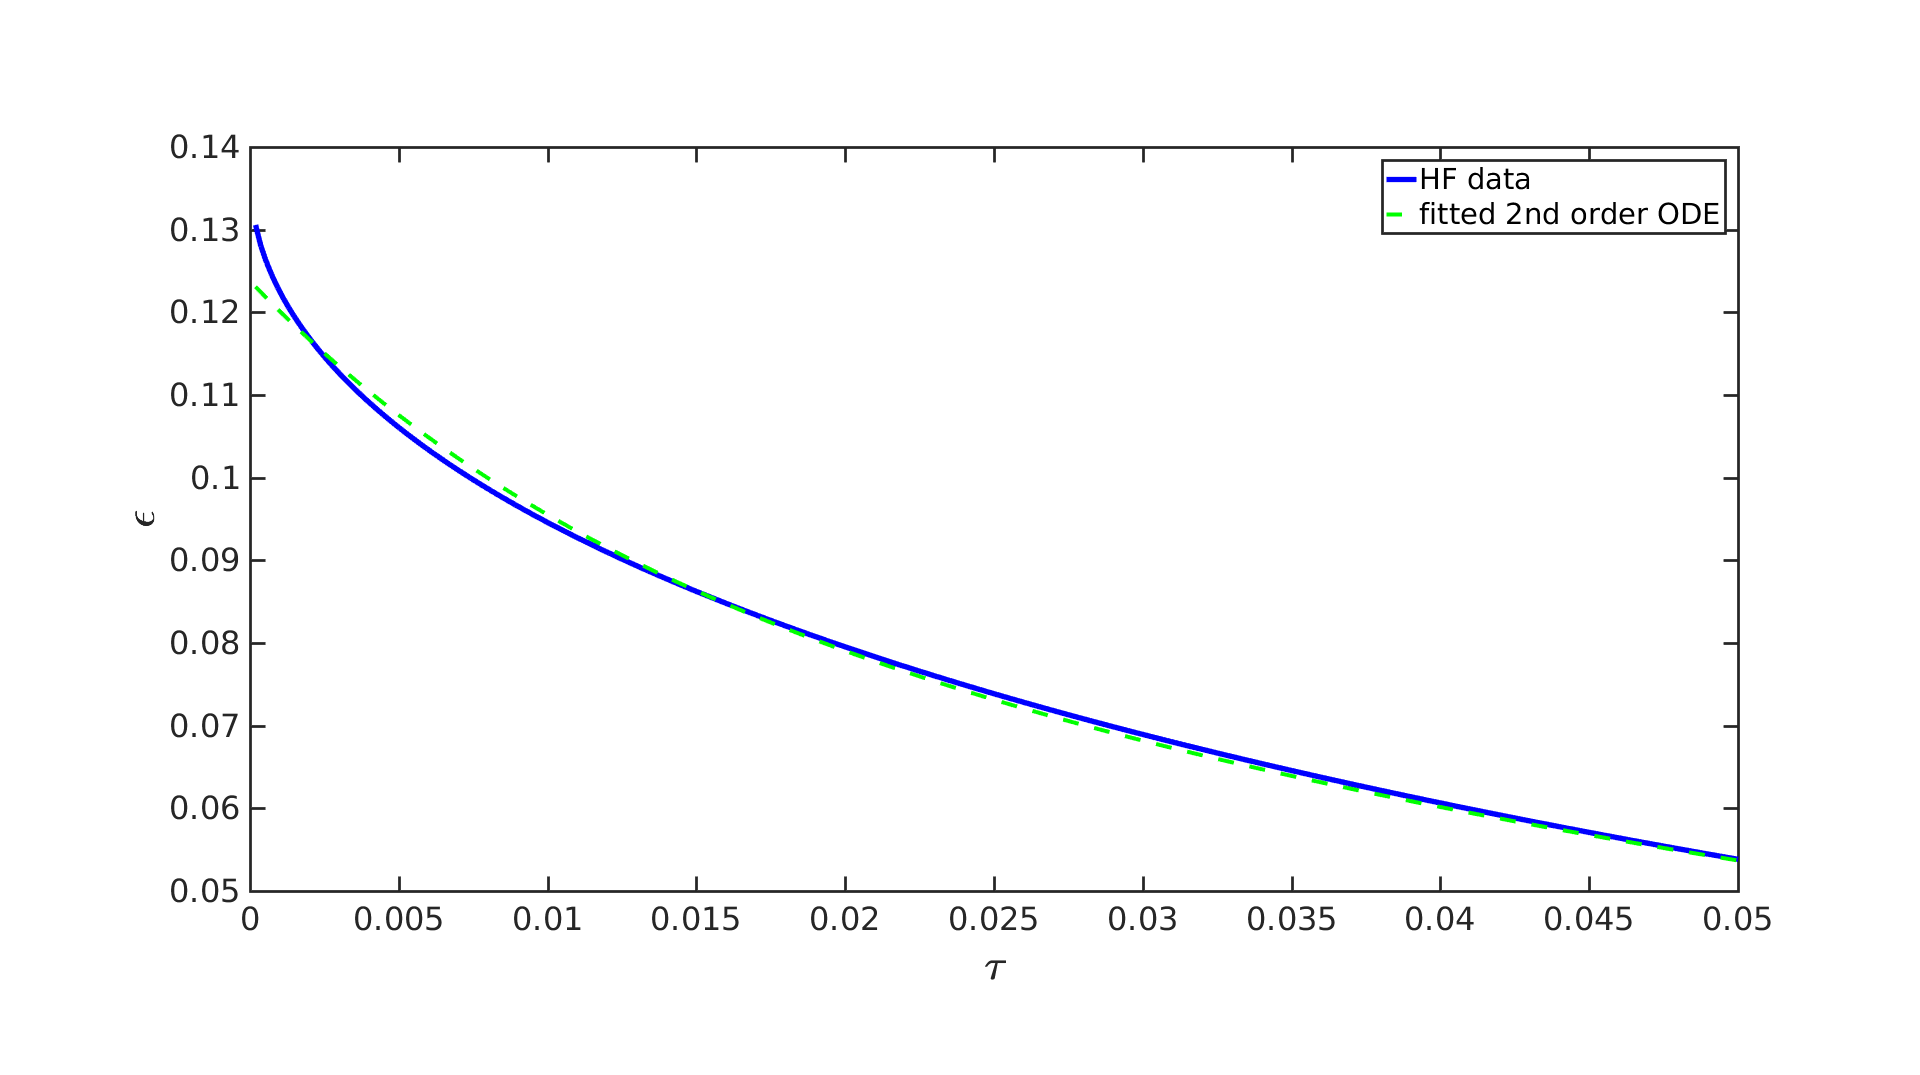
\includegraphics[trim = 1.in 1.in 1.in 1.3in, clip, width=0.5\textwidth]{figs/Iconst_eps_modelfit_2nd_zoom.png}
\end{figure}
\vspace{-0.1in}
Similar results are also expected for step current case, for a small time scale right after $I$ switches.

It should be noted that, for physical point of view, in very short time even the HF might not be represent the reality, due to the simplifying assumptions made to construct HF model.


\vfill
\end{frame}



%===============================================================================
% Slide 01
%===============================================================================
\begin{frame}
\frametitle{Inadequacy Representation: Deterministic}
\textbf{Step current case:}

\vfill

\begin{figure}
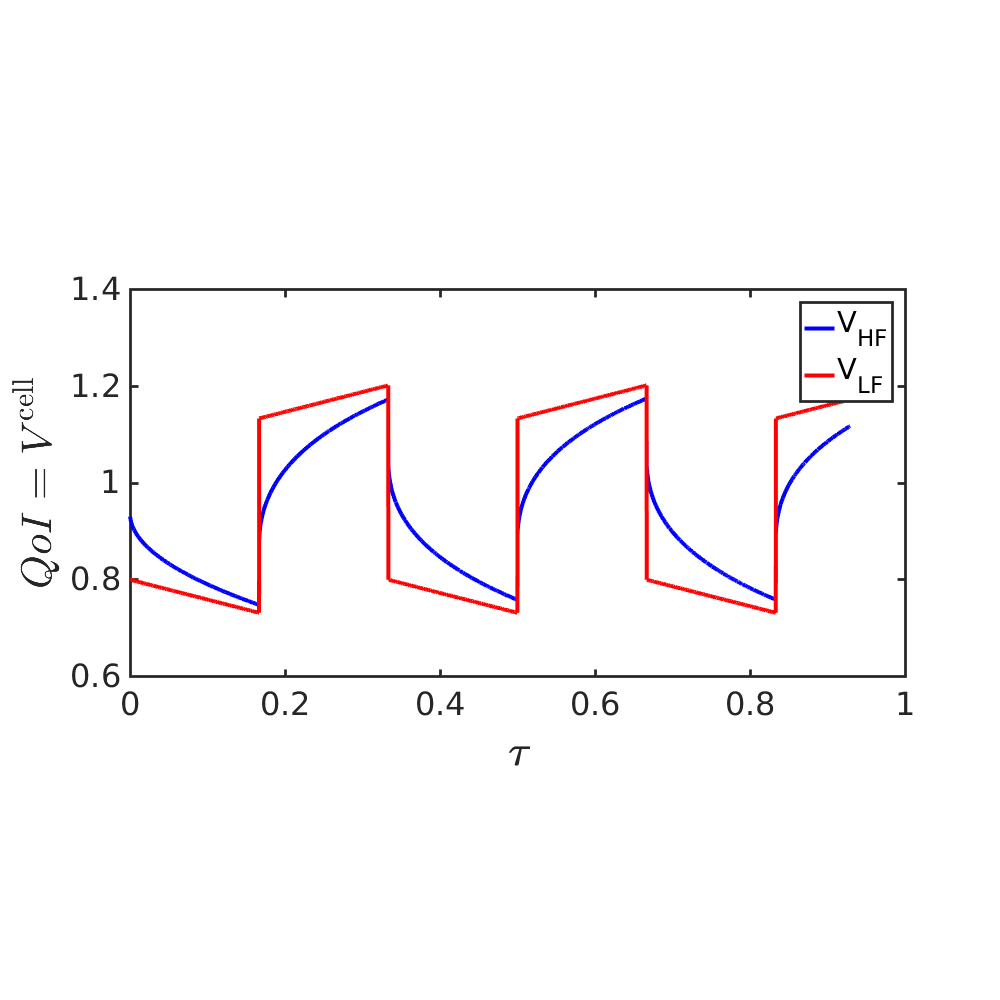
\includegraphics[trim = 0.in  2.3in 0.in 2.8in.in, clip, width=0.5\textwidth]{figs/Istep_V_hf_lf.png}
\end{figure}

\vspace{-0.1in}

Calibrating inadequacy models against HF data: 

\begin{itemize}

\item $\mathcal{P}_1^{\rm d}:   \lambda = 4.2273, \beta = 0.8766, \alpha = 0.2764$

\item $\mathcal{P}_2^{\rm d}:   \lambda = 10.64, \mu = 34.03, \alpha = 9.018, \beta = 23.9858, \rho = 0.3048$

\end{itemize}

\vspace{-0.1in}

\begin{figure}
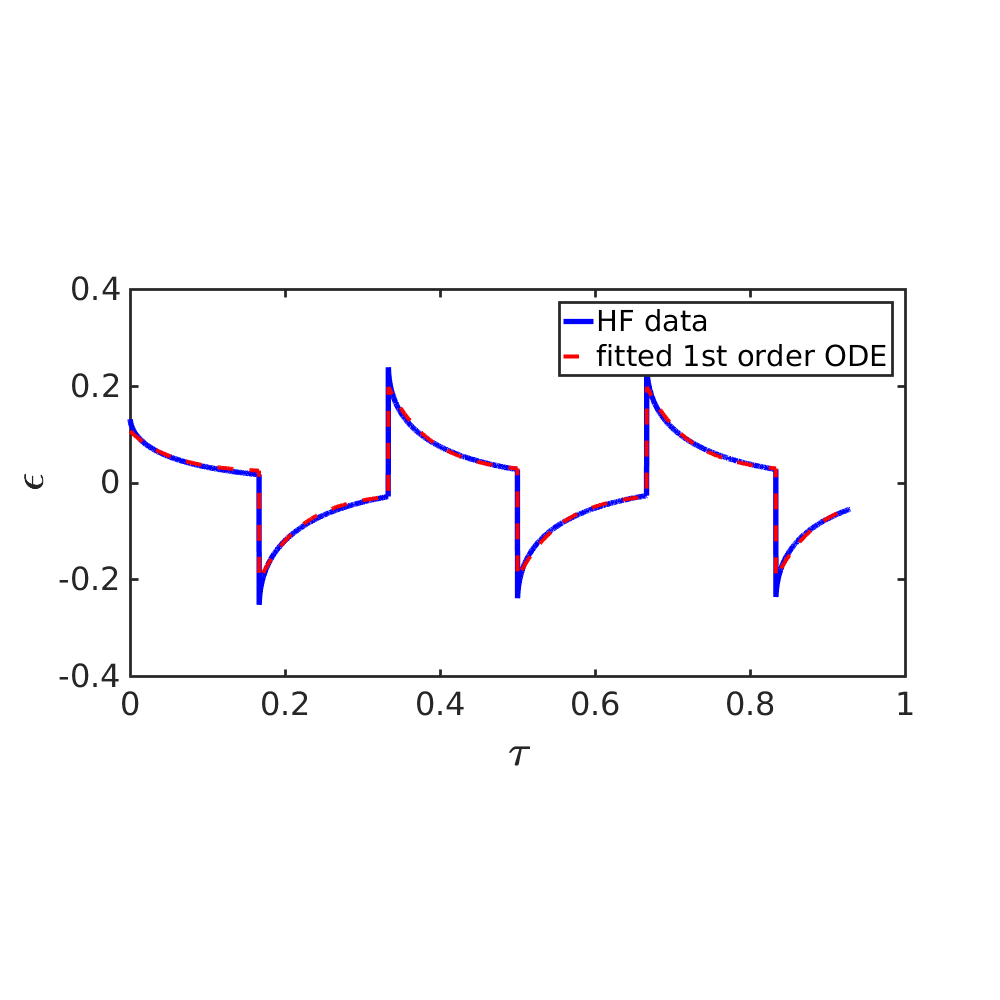
\includegraphics[trim = 0.in  2.3in 0.in 2.8in, clip, width=0.5\textwidth]{figs/Istep_eps_modelfit_1st.png}
~
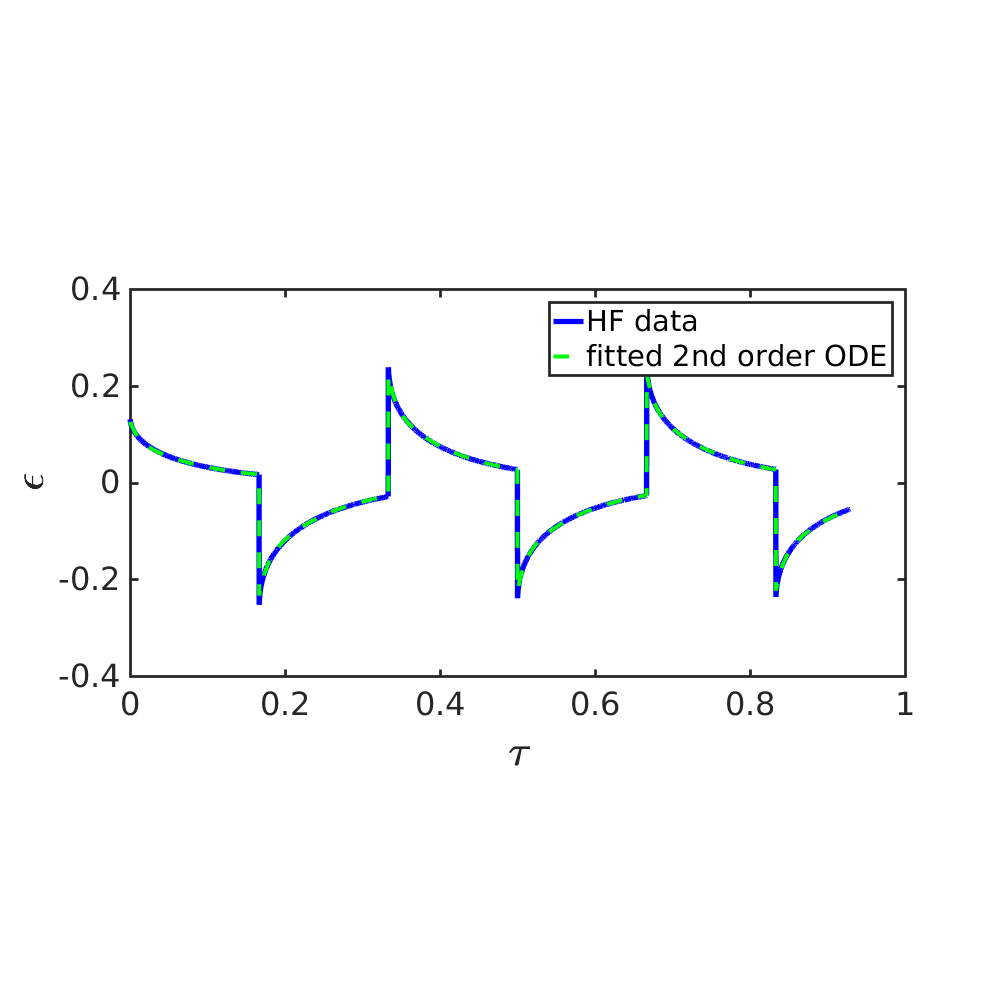
\includegraphics[trim = 0.in  2.3in 0.in 2.8in, clip, width=0.5\textwidth]{figs/Istep_eps_modelfit_2nd.png}
\end{figure}


\vfill
\end{frame}


%===============================================================================
% Slide 01
%===============================================================================
\begin{frame}
\frametitle{Inadequacy Representation: Deterministic}
\textbf{Sinusoidal current case: Low Frequency}

\vfill

\begin{figure}
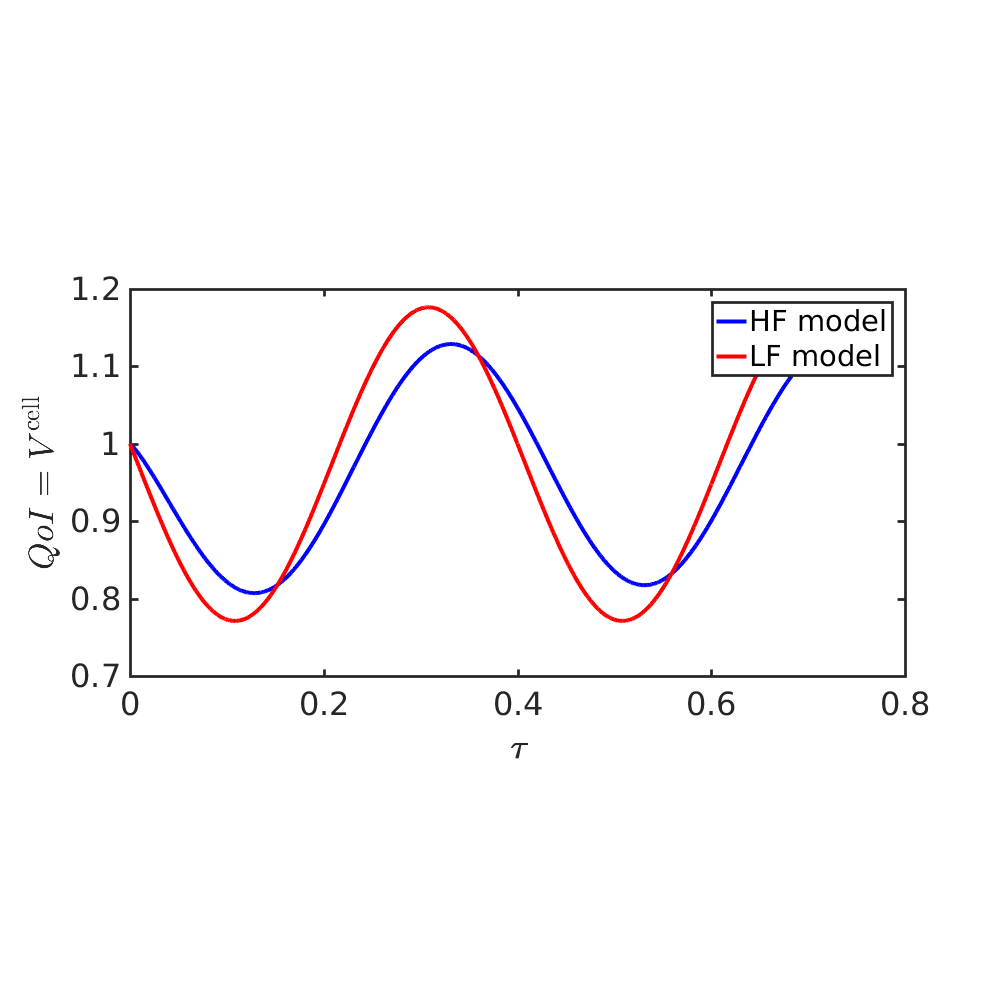
\includegraphics[trim = 0.in  2.3in 0.in 2.8in.in, clip, width=0.5\textwidth]{figs/Isin_low_V_hf_lf.png}
\end{figure}

\vspace{-0.1in}

\begin{figure}
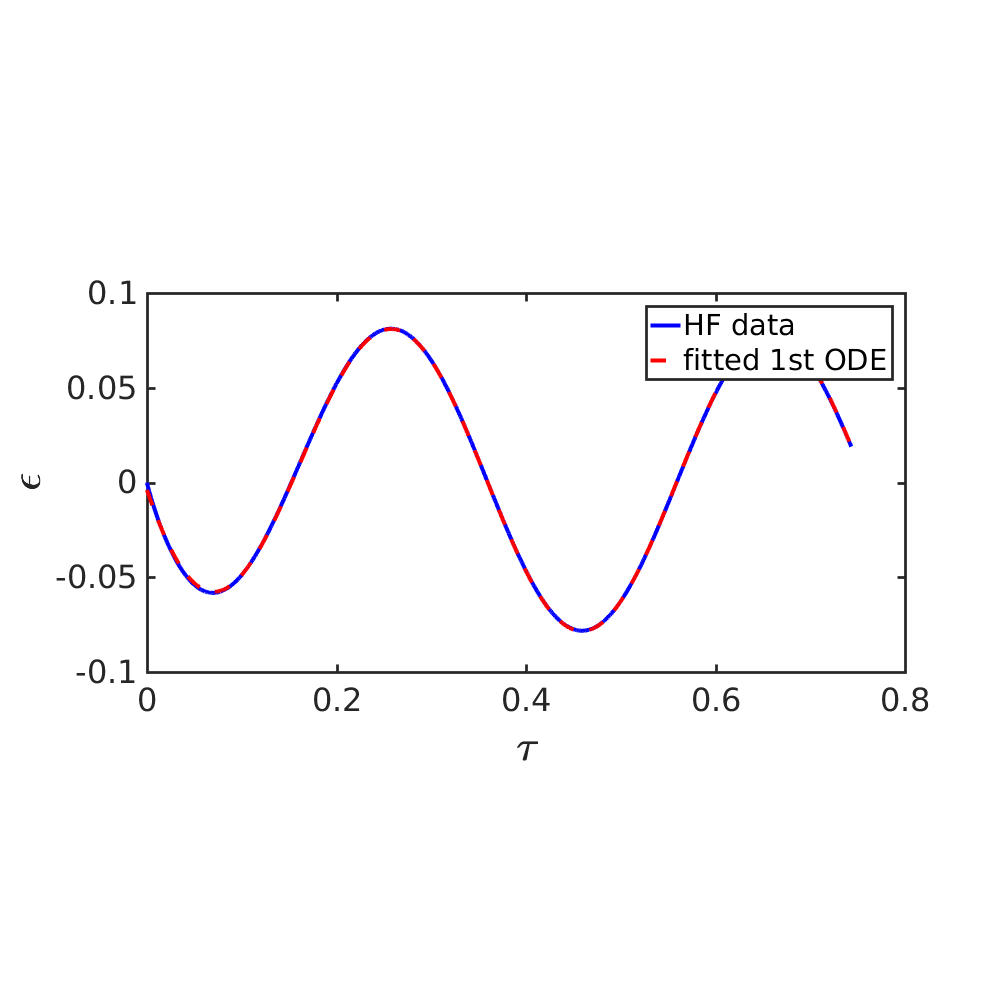
\includegraphics[trim = 0.in  2.3in 0.in 2.8in, clip, width=0.5\textwidth]{figs/Isin_low_fitmodel_1st.png}
~
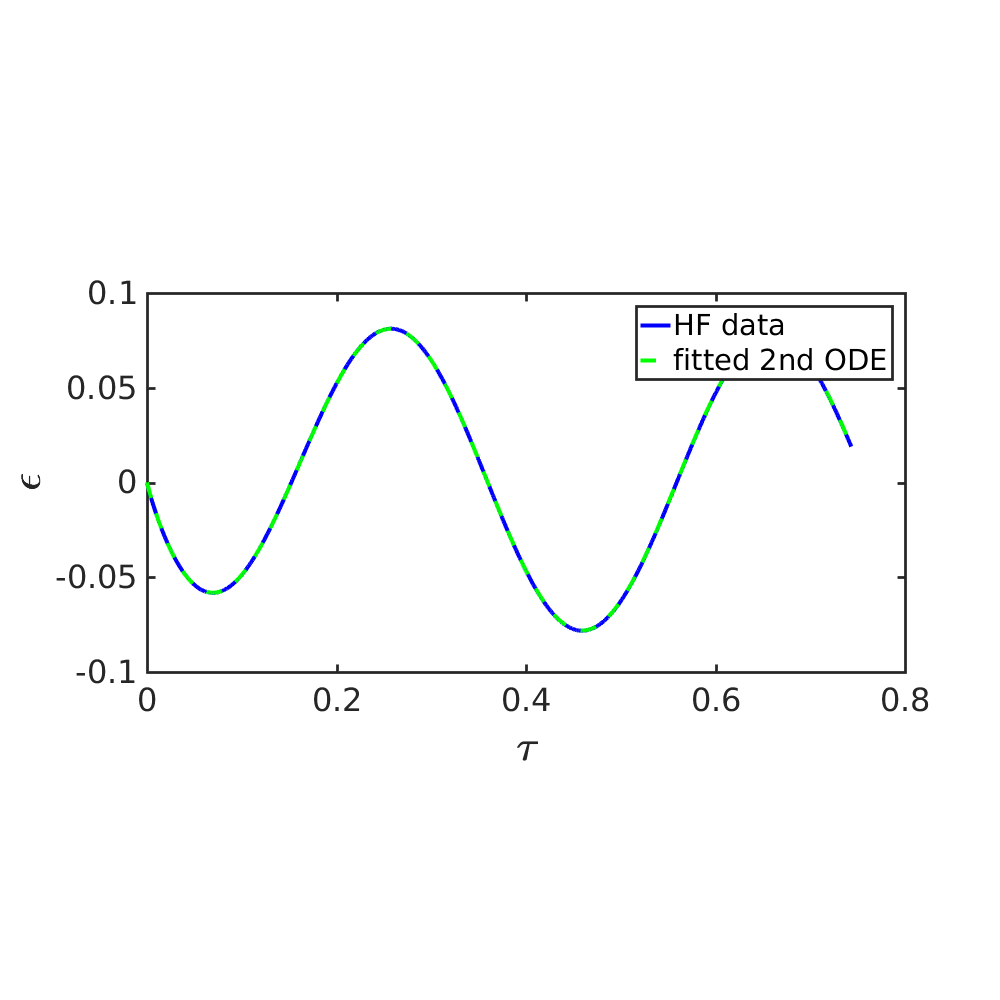
\includegraphics[trim = 0.in  2.3in 0.in 2.8in, clip, width=0.5\textwidth]{figs/Isin_low_fitmodel_2nd.png}
\end{figure}


\vfill
\end{frame}



%===============================================================================
% Slide 01
%===============================================================================
\begin{frame}
\frametitle{Inadequacy Representation: Deterministic}
\textbf{Sinusoidal current case: Intermediate and High Frequency}

\vfill

\vspace{-0.05in}

\begin{figure}
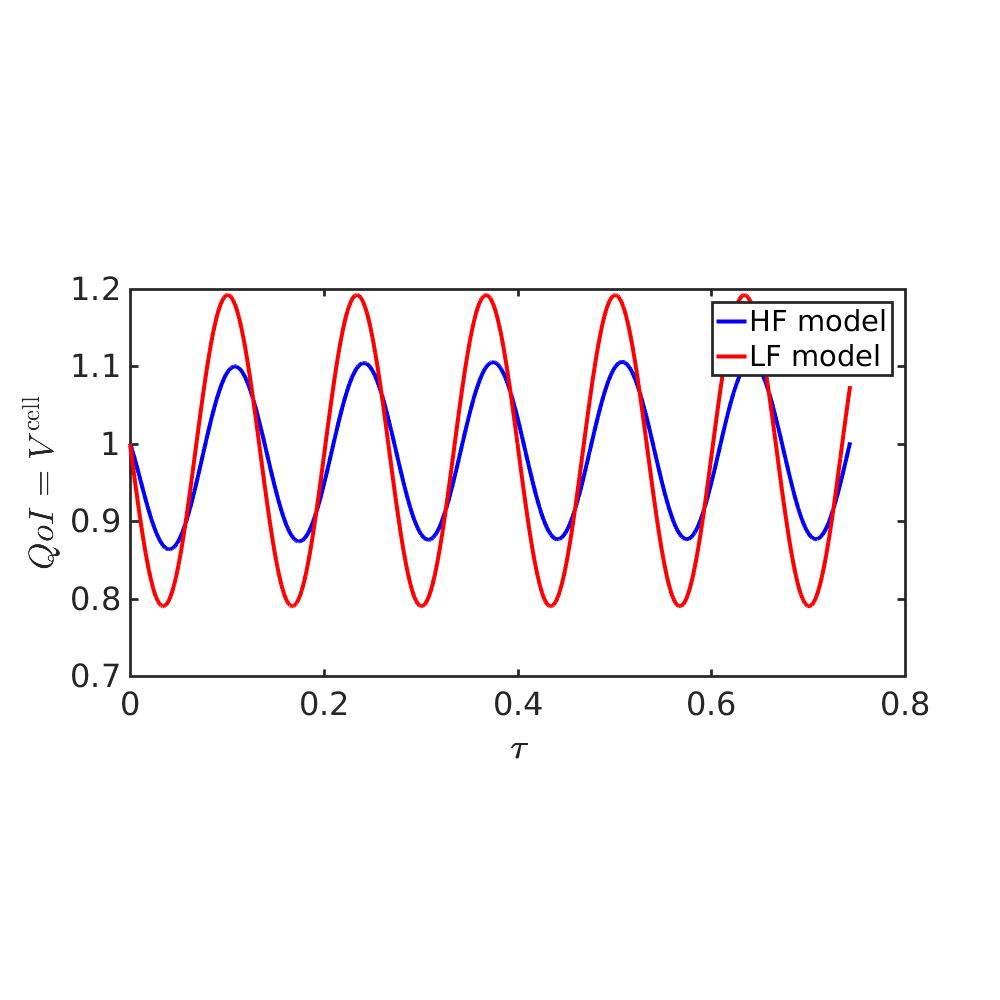
\includegraphics[trim = 0.in  2.3in 0.in 2.8in.in, clip, width=0.45\textwidth]{figs/Isin_int_V_hf_lf.png}
~
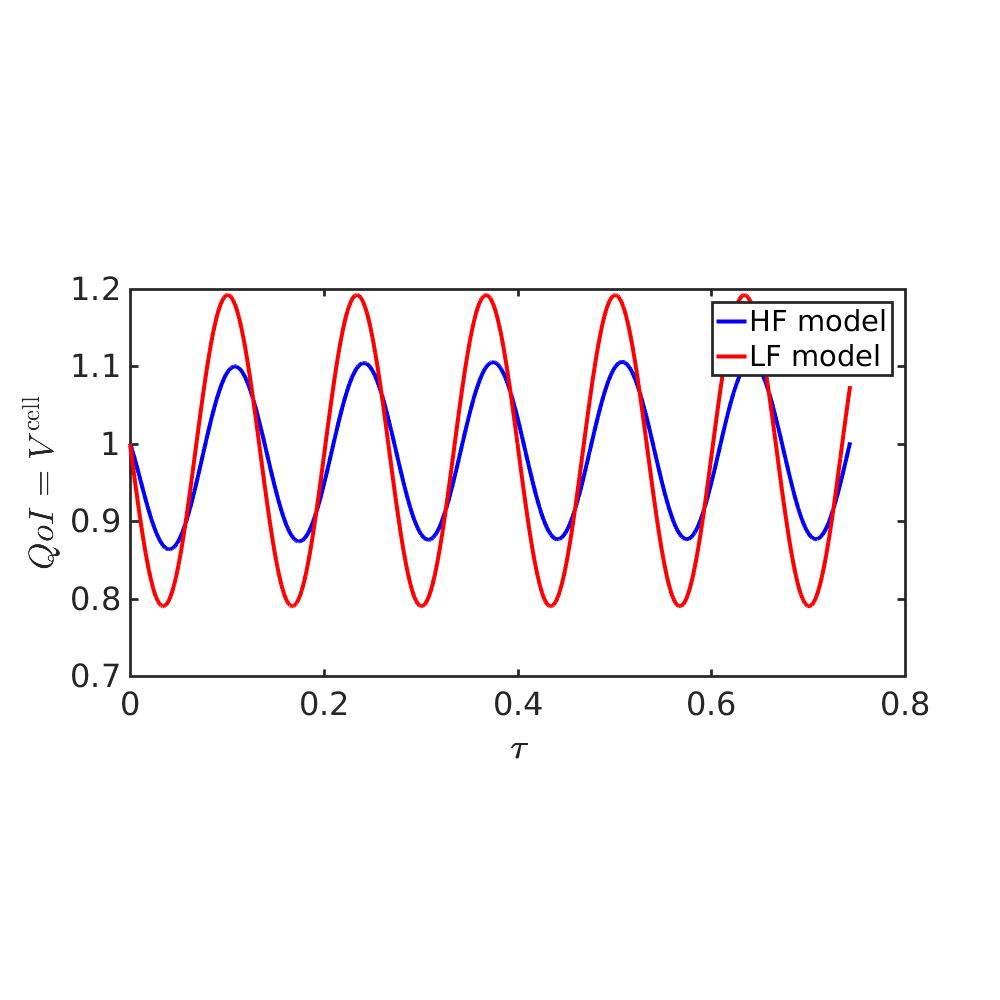
\includegraphics[trim = 0.in  2.3in 0.in 2.8in.in, clip, width=0.45\textwidth]{figs/Isin_high_V_hf_lf.png}
\end{figure}

\vspace{-0.18in}

\begin{figure}
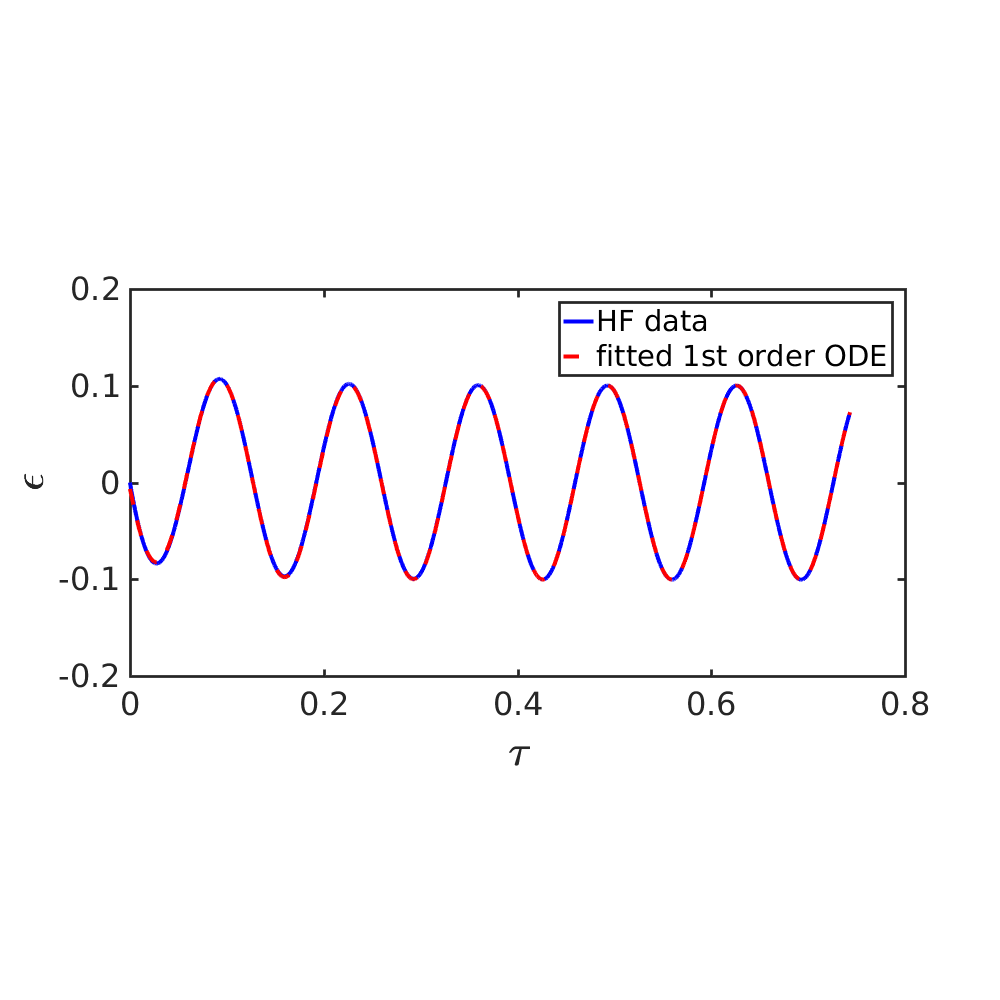
\includegraphics[trim = 0.in  2.3in 0.in 2.8in, clip, width=0.45\textwidth]{figs/Isin_int_epsfit_1st.png}
~
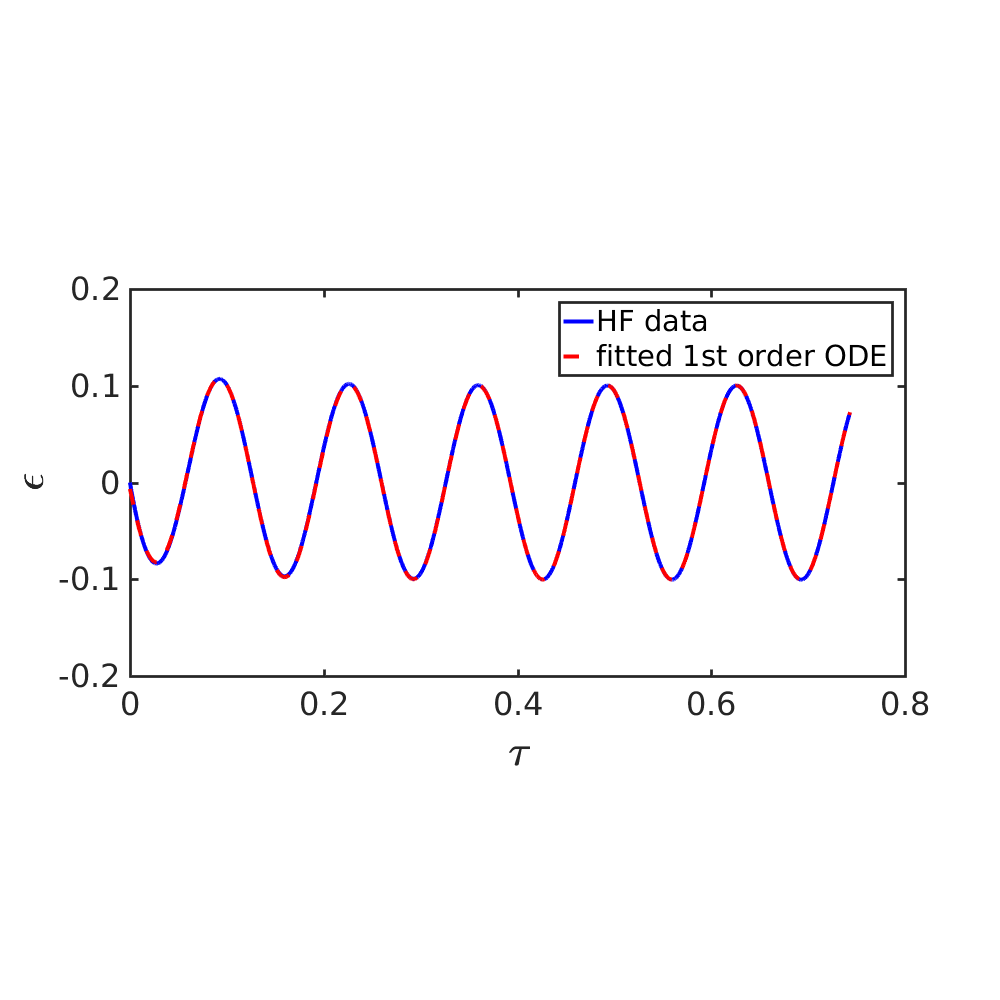
\includegraphics[trim = 0.in  2.3in 0.in 2.8in, clip, width=0.45\textwidth]{figs/Isin_high_epsfit_1st.png}
\end{figure}

\vspace{-0.18in}

\begin{figure}
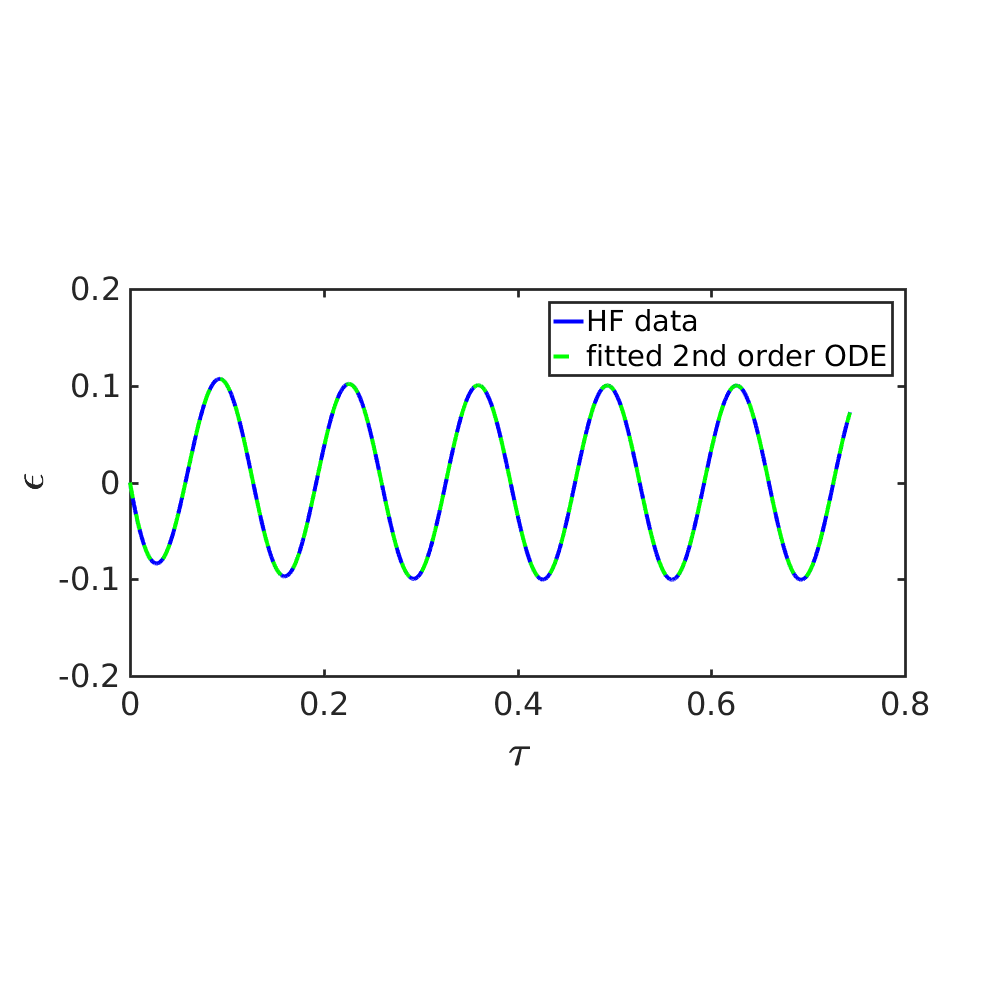
\includegraphics[trim = 0.in  2.3in 0.in 2.8in, clip, width=0.45\textwidth]{figs/Isin_int_epsfit_2nd.png}
~
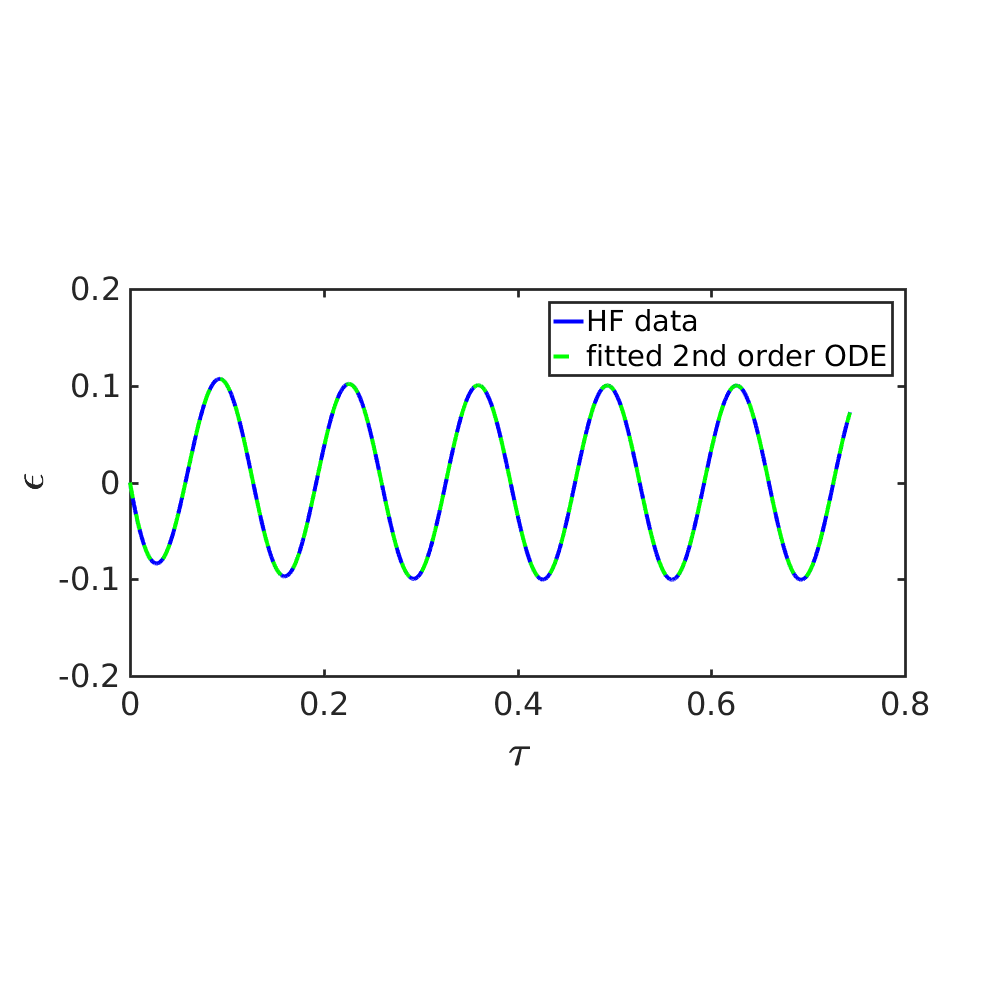
\includegraphics[trim = 0.in  2.3in 0.in 2.8in, clip, width=0.45\textwidth]{figs/Isin_high_epsfit_2nd.png}
\end{figure}


\vfill
\end{frame}




%===============================================================================
% Slide 01
%===============================================================================
\begin{frame}
\frametitle{Inadequacy Representation: Deterministic}

\textbf{Sinusoidal current case: Different current frequencies}


\vfill

\begin{table}
\centering
\begin{tabular}{cc|c|cc|cc}
\cline{3-7}
                                      &         & Low Freq. & Inter Freq. & error$^*$ & High Freq. & error$^*$ \\ \hline
\multicolumn{1}{c|}{} & $\lambda$ & 3.3459 & 3.8389 & -0.147 & 4.7179 & -0.410\\
\multicolumn{1}{c|}{$\mathcal{P}_1^{\rm d}$} & $\beta$ & 0.0932 & 0.134 & -0.440 & 0.035 & 0.624 \\
\multicolumn{1}{c|}{}  & $\alpha$ & -0.2352 & -0.2555 & -0.086	& -0.2746	& -0.167 \\ \hline
\multicolumn{1}{c|}{} & $\lambda$ & 8.8651 &  9.4434  & -0.0652 &  7.6434 & 0.138 \\
\multicolumn{1}{c|}{}  &$\mu	$ & 26.6081 & 29.7492  & -0.118 & 32.298 & -0.214 \\
\multicolumn{1}{c|}{$\mathcal{P}_2^{\rm d}$}  &$\alpha$ & 36.35 & 38.39 & -0.0561 & 40.94	& -0.126  \\
\multicolumn{1}{c|}{}  &$\beta$	& -15.38 &  -18	& -0.17 & -20.93 & -0.361  \\
\multicolumn{1}{c|}{}   &$\rho$	& 0.1415	& 0.2079	& -0.4693	& 0.2801	& -0.979  \\ \hline
\end{tabular}
\\$^*${\small error = relative error wrt parameters of Low Freq}
\end{table}

If we calibrate $\mathcal{P}^{\rm d}$ against HF data obtained from low frequency scenario
\begin{itemize}
\item The deterministic inadequacy representation enables predicting the intermediate frequency scenario. 
\item It break down for predicting the high frequency scenario. 
\end{itemize}

\vfill
\end{frame}


%%%%%%%--------------------------------------------------------------------------------------------------------------------------
\subsection{Stochastic part of inadequacy}
%===============================================================================
% SLIDE 00
%===============================================================================
\begin{frame}
\frametitle{Outline}
\vfill

\vspace{0.7in}
\tableofcontents[currentsection,currentsubsection] 
\vspace{0.7in}

\vfill
\end{frame}




\end{document}
